%-*-latex-*-
\sectionthree{Stack}
\begin{python0}
from solutions import *; clear()
\end{python0}

Recall (see CISS240/245) that a stack is an ADT that looks like
the container for plates at a buffet.
Here's a stack with three values:

\begin{center}
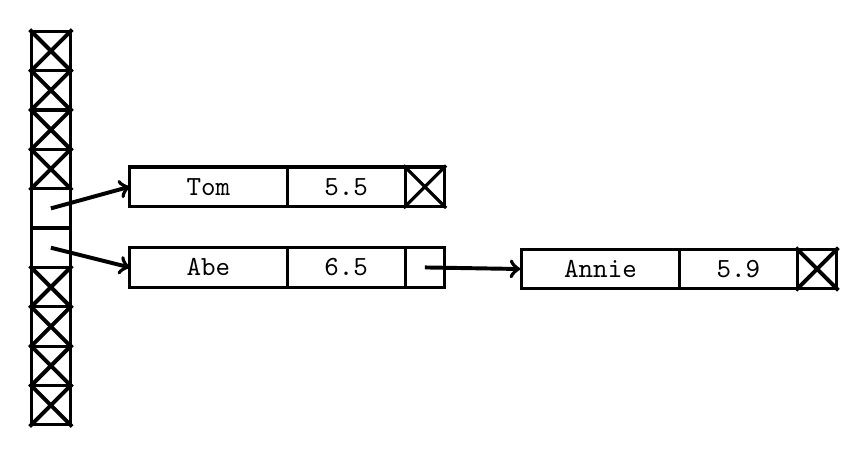
\begin{tikzpicture}
\draw[line width=0.05cm,black] (1.98,0.020000000000000018) to  (2.52,-0.52);
\draw[line width=0.05cm,black] (2.52,0.020000000000000018) to  (1.98,-0.52);
\draw[line width=0.05cm,black] (1.98,-0.48) to  (2.52,-1.02);
\draw[line width=0.05cm,black] (2.52,-0.48) to  (1.98,-1.02);
\draw[line width=0.05cm,black] (1.98,-0.98) to  (2.52,-1.52);
\draw[line width=0.05cm,black] (2.52,-0.98) to  (1.98,-1.52);
\draw[line width=0.05cm,black] (1.98,-1.48) to  (2.52,-2.02);
\draw[line width=0.05cm,black] (2.52,-1.48) to  (1.98,-2.02);

\draw (4.25, -1.975)
  node[draw, line width=0.04cm, , color=black,
       rounded corners=0cm, inner sep=0cm] {

\begin{minipage}[t][0.5cm]{2.0cm}
\mbox{}

\end{minipage}

};\draw (4.25, -1.975) node[color=black] {\texttt{Tom}};
\draw (6.0, -1.975)
  node[draw, line width=0.04cm, , color=black,
       rounded corners=0cm, inner sep=0cm] {

\begin{minipage}[t][0.5cm]{1.5cm}
\mbox{}

\end{minipage}

};\draw (6.0, -1.975) node[color=black] {\texttt{5.5}};
\draw (7.0, -1.975)
  node[draw, line width=0.04cm, , color=black,
       rounded corners=0cm, inner sep=0cm] {

\begin{minipage}[t][0.5cm]{0.5cm}
\mbox{}

\end{minipage}

};\draw[line width=0.05cm,black,->] (2.25,-2.25) to  (3.25,-1.9749999999999999);

\fill[black] (2.25, -2.25) circle (0);
\draw[black] (2.25, -2.25) circle (0.0);\draw[line width=0.04cm,black] (6.73,-1.705) to  (7.27,-2.245);
\draw[line width=0.04cm,black] (7.27,-1.705) to  (6.73,-2.245);

\draw (4.25, -3.0)
  node[draw, line width=0.04cm, , color=black,
       rounded corners=0cm, inner sep=0cm] {

\begin{minipage}[t][0.5cm]{2.0cm}
\mbox{}

\end{minipage}

};\draw (4.25, -3.0) node[color=black] {\texttt{Abe}};
\draw (6.0, -3.0)
  node[draw, line width=0.04cm, , color=black,
       rounded corners=0cm, inner sep=0cm] {

\begin{minipage}[t][0.5cm]{1.5cm}
\mbox{}

\end{minipage}

};\draw (6.0, -3.0) node[color=black] {\texttt{6.5}};
\draw (7.0, -3.0)
  node[draw, line width=0.04cm, , color=black,
       rounded corners=0cm, inner sep=0cm] {

\begin{minipage}[t][0.5cm]{0.5cm}
\mbox{}

\end{minipage}

};\draw[line width=0.05cm,black,->] (2.25,-2.75) to  (3.25,-3.0);

\fill[black] (2.25, -2.75) circle (0);
\draw[black] (2.25, -2.75) circle (0.0);
\draw (9.23, -3.02)
  node[draw, line width=0.04cm, , color=black,
       rounded corners=0cm, inner sep=0cm] {

\begin{minipage}[t][0.5cm]{2.0cm}
\mbox{}

\end{minipage}

};\draw (9.23, -3.02) node[color=black] {\texttt{Annie}};
\draw (10.98, -3.02)
  node[draw, line width=0.04cm, , color=black,
       rounded corners=0cm, inner sep=0cm] {

\begin{minipage}[t][0.5cm]{1.5cm}
\mbox{}

\end{minipage}

};\draw (10.98, -3.02) node[color=black] {\texttt{5.9}};
\draw (11.98, -3.02)
  node[draw, line width=0.04cm, , color=black,
       rounded corners=0cm, inner sep=0cm] {

\begin{minipage}[t][0.5cm]{0.5cm}
\mbox{}

\end{minipage}

};\draw[line width=0.05cm,black] (11.71,-2.75) to  (12.25,-3.29);
\draw[line width=0.05cm,black] (12.25,-2.75) to  (11.71,-3.29);
\draw[line width=0.05cm,black,->] (7.0,-3.0) to  (8.21,-3.0199999999999996);

\fill[black] (7.0, -3.0) circle (0);
\draw[black] (7.0, -3.0) circle (0.0);\draw[line width=0.05cm,black] (1.98,-2.98) to  (2.52,-3.52);
\draw[line width=0.05cm,black] (2.52,-2.98) to  (1.98,-3.52);
\draw[line width=0.05cm,black] (1.98,-3.4800000000000004) to  (2.52,-4.02);
\draw[line width=0.05cm,black] (2.52,-3.4800000000000004) to  (1.98,-4.02);
\draw[line width=0.05cm,black] (1.98,-3.9800000000000004) to  (2.52,-4.52);
\draw[line width=0.05cm,black] (2.52,-3.9800000000000004) to  (1.98,-4.52);
\draw[line width=0.05cm,black] (1.98,-4.48) to  (2.52,-5.02);
\draw[line width=0.05cm,black] (2.52,-4.48) to  (1.98,-5.02);

\draw (2.25, -0.25)
  node[draw, line width=0.04cm, , color=black,
       rounded corners=0cm, inner sep=0cm] {

\begin{minipage}[t][0.5cm]{0.5cm}
\mbox{}

\end{minipage}

};
\draw (2.25, -0.75)
  node[draw, line width=0.04cm, , color=black,
       rounded corners=0cm, inner sep=0cm] {

\begin{minipage}[t][0.5cm]{0.5cm}
\mbox{}

\end{minipage}

};
\draw (2.25, -1.25)
  node[draw, line width=0.04cm, , color=black,
       rounded corners=0cm, inner sep=0cm] {

\begin{minipage}[t][0.5cm]{0.5cm}
\mbox{}

\end{minipage}

};
\draw (2.25, -1.75)
  node[draw, line width=0.04cm, , color=black,
       rounded corners=0cm, inner sep=0cm] {

\begin{minipage}[t][0.5cm]{0.5cm}
\mbox{}

\end{minipage}

};
\draw (2.25, -2.25)
  node[draw, line width=0.04cm, , color=black,
       rounded corners=0cm, inner sep=0cm] {

\begin{minipage}[t][0.5cm]{0.5cm}
\mbox{}

\end{minipage}

};
\draw (2.25, -2.75)
  node[draw, line width=0.04cm, , color=black,
       rounded corners=0cm, inner sep=0cm] {

\begin{minipage}[t][0.5cm]{0.5cm}
\mbox{}

\end{minipage}

};
\draw (2.25, -3.25)
  node[draw, line width=0.04cm, , color=black,
       rounded corners=0cm, inner sep=0cm] {

\begin{minipage}[t][0.5cm]{0.5cm}
\mbox{}

\end{minipage}

};
\draw (2.25, -3.75)
  node[draw, line width=0.04cm, , color=black,
       rounded corners=0cm, inner sep=0cm] {

\begin{minipage}[t][0.5cm]{0.5cm}
\mbox{}

\end{minipage}

};
\draw (2.25, -4.25)
  node[draw, line width=0.04cm, , color=black,
       rounded corners=0cm, inner sep=0cm] {

\begin{minipage}[t][0.5cm]{0.5cm}
\mbox{}

\end{minipage}

};
\draw (2.25, -4.75)
  node[draw, line width=0.04cm, , color=black,
       rounded corners=0cm, inner sep=0cm] {

\begin{minipage}[t][0.5cm]{0.5cm}
\mbox{}

\end{minipage}

};
\end{tikzpicture}

\end{center}



If I put a 5 into the stack, it looks like this:

\begin{center}
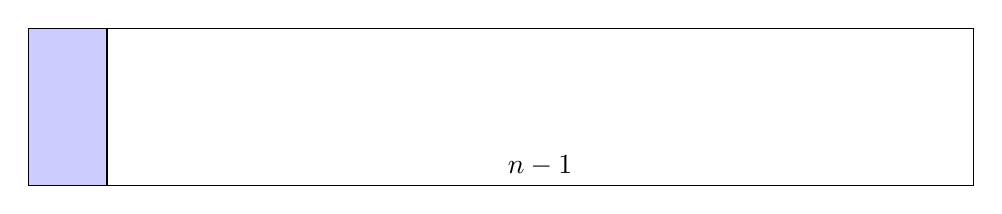
\begin{tikzpicture}

\draw (6.0, 1.0)
  node[draw, , , color=black,
       rounded corners=0cm, inner sep=0cm] {

\begin{minipage}[t][2cm]{12cm}
\mbox{}

\end{minipage}

};
\draw (0.5, 1.0)
  node[fill=blue!20!white,rounded corners=0cm,inner sep=0cm] {

\begin{minipage}[t][2cm]{1cm}
\mbox{}

\end{minipage}

};
\draw (0.5, 1.0)
  node[draw, , , color=black,
       rounded corners=0cm, inner sep=0cm] {

\begin{minipage}[t][2cm]{1cm}
\mbox{}

\end{minipage}

};
\draw (6.5, 0.25)
  node[draw=none, line width=0cm, , color=black,
       rounded corners=0cm, inner sep=0cm] {

\begin{minipage}[t][0.1cm]{0.1cm}
\mbox{}

\end{minipage}

};\draw (6.5, 0.25) node[color=black] {$n - 1$};
\end{tikzpicture}

\end{center}



If I put a 4 into the stack, then it looks like this:

\begin{center}
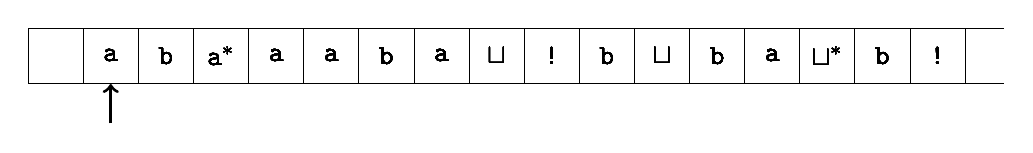
\begin{tikzpicture}

\draw (0.35, 0.35)
  node[draw, line width=0.01cm, , color=black,
       rounded corners=0cm, inner sep=0cm] {

\begin{minipage}[t][0.7cm]{0.7cm}
\mbox{}

\end{minipage}

};\draw (0.35, 0.35) node[color=black] {\texttt{\DOLLAR}};
\draw (1.0499999999999998, 0.35)
  node[draw, line width=0.01cm, , color=black,
       rounded corners=0cm, inner sep=0cm] {

\begin{minipage}[t][0.7cm]{0.7cm}
\mbox{}

\end{minipage}

};\draw (1.0499999999999998, 0.35) node[color=black] {\texttt{a}};
\draw (1.7499999999999998, 0.35)
  node[draw, line width=0.01cm, , color=black,
       rounded corners=0cm, inner sep=0cm] {

\begin{minipage}[t][0.7cm]{0.7cm}
\mbox{}

\end{minipage}

};\draw (1.7499999999999998, 0.35) node[color=black] {\texttt{b}};
\draw (2.4499999999999997, 0.35)
  node[draw, line width=0.01cm, , color=black,
       rounded corners=0cm, inner sep=0cm] {

\begin{minipage}[t][0.7cm]{0.7cm}
\mbox{}

\end{minipage}

};\draw (2.4499999999999997, 0.35) node[color=black] {\texttt{a$^*$}};
\draw (3.15, 0.35)
  node[draw, line width=0.01cm, , color=black,
       rounded corners=0cm, inner sep=0cm] {

\begin{minipage}[t][0.7cm]{0.7cm}
\mbox{}

\end{minipage}

};\draw (3.15, 0.35) node[color=black] {\texttt{a}};
\draw (3.85, 0.35)
  node[draw, line width=0.01cm, , color=black,
       rounded corners=0cm, inner sep=0cm] {

\begin{minipage}[t][0.7cm]{0.7cm}
\mbox{}

\end{minipage}

};\draw (3.85, 0.35) node[color=black] {\texttt{a}};
\draw (4.550000000000001, 0.35)
  node[draw, line width=0.01cm, , color=black,
       rounded corners=0cm, inner sep=0cm] {

\begin{minipage}[t][0.7cm]{0.7cm}
\mbox{}

\end{minipage}

};\draw (4.550000000000001, 0.35) node[color=black] {\texttt{b}};
\draw (5.25, 0.35)
  node[draw, line width=0.01cm, , color=black,
       rounded corners=0cm, inner sep=0cm] {

\begin{minipage}[t][0.7cm]{0.7cm}
\mbox{}

\end{minipage}

};\draw (5.25, 0.35) node[color=black] {\texttt{a}};
\draw (5.950000000000001, 0.35)
  node[draw, line width=0.01cm, , color=black,
       rounded corners=0cm, inner sep=0cm] {

\begin{minipage}[t][0.7cm]{0.7cm}
\mbox{}

\end{minipage}

};\draw (5.950000000000001, 0.35) node[color=black] {\texttt{$\sqcup$}};
\draw (6.65, 0.35)
  node[draw, line width=0.01cm, , color=black,
       rounded corners=0cm, inner sep=0cm] {

\begin{minipage}[t][0.7cm]{0.7cm}
\mbox{}

\end{minipage}

};\draw (6.65, 0.35) node[color=black] {\texttt{!}};
\draw (7.350000000000001, 0.35)
  node[draw, line width=0.01cm, , color=black,
       rounded corners=0cm, inner sep=0cm] {

\begin{minipage}[t][0.7cm]{0.7cm}
\mbox{}

\end{minipage}

};\draw (7.350000000000001, 0.35) node[color=black] {\texttt{b}};
\draw (8.05, 0.35)
  node[draw, line width=0.01cm, , color=black,
       rounded corners=0cm, inner sep=0cm] {

\begin{minipage}[t][0.7cm]{0.7cm}
\mbox{}

\end{minipage}

};\draw (8.05, 0.35) node[color=black] {\texttt{$\sqcup$}};
\draw (8.75, 0.35)
  node[draw, line width=0.01cm, , color=black,
       rounded corners=0cm, inner sep=0cm] {

\begin{minipage}[t][0.7cm]{0.7cm}
\mbox{}

\end{minipage}

};\draw (8.75, 0.35) node[color=black] {\texttt{b}};
\draw (9.45, 0.35)
  node[draw, line width=0.01cm, , color=black,
       rounded corners=0cm, inner sep=0cm] {

\begin{minipage}[t][0.7cm]{0.7cm}
\mbox{}

\end{minipage}

};\draw (9.45, 0.35) node[color=black] {\texttt{a}};
\draw (10.149999999999999, 0.35)
  node[draw, line width=0.01cm, , color=black,
       rounded corners=0cm, inner sep=0cm] {

\begin{minipage}[t][0.7cm]{0.7cm}
\mbox{}

\end{minipage}

};\draw (10.149999999999999, 0.35) node[color=black] {\texttt{$\sqcup^*$}};
\draw (10.849999999999998, 0.35)
  node[draw, line width=0.01cm, , color=black,
       rounded corners=0cm, inner sep=0cm] {

\begin{minipage}[t][0.7cm]{0.7cm}
\mbox{}

\end{minipage}

};\draw (10.849999999999998, 0.35) node[color=black] {\texttt{b}};
\draw (11.549999999999997, 0.35)
  node[draw, line width=0.01cm, , color=black,
       rounded corners=0cm, inner sep=0cm] {

\begin{minipage}[t][0.7cm]{0.7cm}
\mbox{}

\end{minipage}

};\draw (11.549999999999997, 0.35) node[color=black] {\texttt{!}};
\draw (0.35, 0.35)
  node[draw, line width=0.01cm, , color=black,
       rounded corners=0cm, inner sep=0cm] {

\begin{minipage}[t][0.7cm]{0.7cm}
\mbox{}

\end{minipage}

};\draw (0.35, 0.35) node[color=black] {\texttt{\DOLLAR}};
\draw (1.0499999999999998, 0.35)
  node[draw, line width=0.01cm, , color=black,
       rounded corners=0cm, inner sep=0cm] {

\begin{minipage}[t][0.7cm]{0.7cm}
\mbox{}

\end{minipage}

};\draw (1.0499999999999998, 0.35) node[color=black] {\texttt{a}};
\draw (1.7499999999999998, 0.35)
  node[draw, line width=0.01cm, , color=black,
       rounded corners=0cm, inner sep=0cm] {

\begin{minipage}[t][0.7cm]{0.7cm}
\mbox{}

\end{minipage}

};\draw (1.7499999999999998, 0.35) node[color=black] {\texttt{b}};
\draw (2.4499999999999997, 0.35)
  node[draw, line width=0.01cm, , color=black,
       rounded corners=0cm, inner sep=0cm] {

\begin{minipage}[t][0.7cm]{0.7cm}
\mbox{}

\end{minipage}

};\draw (2.4499999999999997, 0.35) node[color=black] {\texttt{a$^*$}};
\draw (3.15, 0.35)
  node[draw, line width=0.01cm, , color=black,
       rounded corners=0cm, inner sep=0cm] {

\begin{minipage}[t][0.7cm]{0.7cm}
\mbox{}

\end{minipage}

};\draw (3.15, 0.35) node[color=black] {\texttt{a}};
\draw (3.85, 0.35)
  node[draw, line width=0.01cm, , color=black,
       rounded corners=0cm, inner sep=0cm] {

\begin{minipage}[t][0.7cm]{0.7cm}
\mbox{}

\end{minipage}

};\draw (3.85, 0.35) node[color=black] {\texttt{a}};
\draw (4.550000000000001, 0.35)
  node[draw, line width=0.01cm, , color=black,
       rounded corners=0cm, inner sep=0cm] {

\begin{minipage}[t][0.7cm]{0.7cm}
\mbox{}

\end{minipage}

};\draw (4.550000000000001, 0.35) node[color=black] {\texttt{b}};
\draw (5.25, 0.35)
  node[draw, line width=0.01cm, , color=black,
       rounded corners=0cm, inner sep=0cm] {

\begin{minipage}[t][0.7cm]{0.7cm}
\mbox{}

\end{minipage}

};\draw (5.25, 0.35) node[color=black] {\texttt{a}};
\draw (5.950000000000001, 0.35)
  node[draw, line width=0.01cm, , color=black,
       rounded corners=0cm, inner sep=0cm] {

\begin{minipage}[t][0.7cm]{0.7cm}
\mbox{}

\end{minipage}

};\draw (5.950000000000001, 0.35) node[color=black] {\texttt{$\sqcup$}};
\draw (6.65, 0.35)
  node[draw, line width=0.01cm, , color=black,
       rounded corners=0cm, inner sep=0cm] {

\begin{minipage}[t][0.7cm]{0.7cm}
\mbox{}

\end{minipage}

};\draw (6.65, 0.35) node[color=black] {\texttt{!}};
\draw (7.350000000000001, 0.35)
  node[draw, line width=0.01cm, , color=black,
       rounded corners=0cm, inner sep=0cm] {

\begin{minipage}[t][0.7cm]{0.7cm}
\mbox{}

\end{minipage}

};\draw (7.350000000000001, 0.35) node[color=black] {\texttt{b}};
\draw (8.05, 0.35)
  node[draw, line width=0.01cm, , color=black,
       rounded corners=0cm, inner sep=0cm] {

\begin{minipage}[t][0.7cm]{0.7cm}
\mbox{}

\end{minipage}

};\draw (8.05, 0.35) node[color=black] {\texttt{$\sqcup$}};
\draw (8.75, 0.35)
  node[draw, line width=0.01cm, , color=black,
       rounded corners=0cm, inner sep=0cm] {

\begin{minipage}[t][0.7cm]{0.7cm}
\mbox{}

\end{minipage}

};\draw (8.75, 0.35) node[color=black] {\texttt{b}};
\draw (9.45, 0.35)
  node[draw, line width=0.01cm, , color=black,
       rounded corners=0cm, inner sep=0cm] {

\begin{minipage}[t][0.7cm]{0.7cm}
\mbox{}

\end{minipage}

};\draw (9.45, 0.35) node[color=black] {\texttt{a}};
\draw (10.149999999999999, 0.35)
  node[draw, line width=0.01cm, , color=black,
       rounded corners=0cm, inner sep=0cm] {

\begin{minipage}[t][0.7cm]{0.7cm}
\mbox{}

\end{minipage}

};\draw (10.149999999999999, 0.35) node[color=black] {\texttt{$\sqcup^*$}};
\draw (10.849999999999998, 0.35)
  node[draw, line width=0.01cm, , color=black,
       rounded corners=0cm, inner sep=0cm] {

\begin{minipage}[t][0.7cm]{0.7cm}
\mbox{}

\end{minipage}

};\draw (10.849999999999998, 0.35) node[color=black] {\texttt{b}};
\draw (11.549999999999997, 0.35)
  node[draw, line width=0.01cm, , color=black,
       rounded corners=0cm, inner sep=0cm] {

\begin{minipage}[t][0.7cm]{0.7cm}
\mbox{}

\end{minipage}

};\draw (11.549999999999997, 0.35) node[color=black] {\texttt{!}};
\draw (0.35, 0.35)
  node[draw, line width=0.01cm, , color=black,
       rounded corners=0cm, inner sep=0cm] {

\begin{minipage}[t][0.7cm]{0.7cm}
\mbox{}

\end{minipage}

};\draw (0.35, 0.35) node[color=black] {\texttt{\DOLLAR}};
\draw (1.0499999999999998, 0.35)
  node[draw, line width=0.01cm, , color=black,
       rounded corners=0cm, inner sep=0cm] {

\begin{minipage}[t][0.7cm]{0.7cm}
\mbox{}

\end{minipage}

};\draw (1.0499999999999998, 0.35) node[color=black] {\texttt{a}};
\draw (1.7499999999999998, 0.35)
  node[draw, line width=0.01cm, , color=black,
       rounded corners=0cm, inner sep=0cm] {

\begin{minipage}[t][0.7cm]{0.7cm}
\mbox{}

\end{minipage}

};\draw (1.7499999999999998, 0.35) node[color=black] {\texttt{b}};
\draw (2.4499999999999997, 0.35)
  node[draw, line width=0.01cm, , color=black,
       rounded corners=0cm, inner sep=0cm] {

\begin{minipage}[t][0.7cm]{0.7cm}
\mbox{}

\end{minipage}

};\draw (2.4499999999999997, 0.35) node[color=black] {\texttt{a$^*$}};
\draw (3.15, 0.35)
  node[draw, line width=0.01cm, , color=black,
       rounded corners=0cm, inner sep=0cm] {

\begin{minipage}[t][0.7cm]{0.7cm}
\mbox{}

\end{minipage}

};\draw (3.15, 0.35) node[color=black] {\texttt{a}};
\draw (3.85, 0.35)
  node[draw, line width=0.01cm, , color=black,
       rounded corners=0cm, inner sep=0cm] {

\begin{minipage}[t][0.7cm]{0.7cm}
\mbox{}

\end{minipage}

};\draw (3.85, 0.35) node[color=black] {\texttt{a}};
\draw (4.550000000000001, 0.35)
  node[draw, line width=0.01cm, , color=black,
       rounded corners=0cm, inner sep=0cm] {

\begin{minipage}[t][0.7cm]{0.7cm}
\mbox{}

\end{minipage}

};\draw (4.550000000000001, 0.35) node[color=black] {\texttt{b}};
\draw (5.25, 0.35)
  node[draw, line width=0.01cm, , color=black,
       rounded corners=0cm, inner sep=0cm] {

\begin{minipage}[t][0.7cm]{0.7cm}
\mbox{}

\end{minipage}

};\draw (5.25, 0.35) node[color=black] {\texttt{a}};
\draw (5.950000000000001, 0.35)
  node[draw, line width=0.01cm, , color=black,
       rounded corners=0cm, inner sep=0cm] {

\begin{minipage}[t][0.7cm]{0.7cm}
\mbox{}

\end{minipage}

};\draw (5.950000000000001, 0.35) node[color=black] {\texttt{$\sqcup$}};
\draw (6.65, 0.35)
  node[draw, line width=0.01cm, , color=black,
       rounded corners=0cm, inner sep=0cm] {

\begin{minipage}[t][0.7cm]{0.7cm}
\mbox{}

\end{minipage}

};\draw (6.65, 0.35) node[color=black] {\texttt{!}};
\draw (7.350000000000001, 0.35)
  node[draw, line width=0.01cm, , color=black,
       rounded corners=0cm, inner sep=0cm] {

\begin{minipage}[t][0.7cm]{0.7cm}
\mbox{}

\end{minipage}

};\draw (7.350000000000001, 0.35) node[color=black] {\texttt{b}};
\draw (8.05, 0.35)
  node[draw, line width=0.01cm, , color=black,
       rounded corners=0cm, inner sep=0cm] {

\begin{minipage}[t][0.7cm]{0.7cm}
\mbox{}

\end{minipage}

};\draw (8.05, 0.35) node[color=black] {\texttt{$\sqcup$}};
\draw (8.75, 0.35)
  node[draw, line width=0.01cm, , color=black,
       rounded corners=0cm, inner sep=0cm] {

\begin{minipage}[t][0.7cm]{0.7cm}
\mbox{}

\end{minipage}

};\draw (8.75, 0.35) node[color=black] {\texttt{b}};
\draw (9.45, 0.35)
  node[draw, line width=0.01cm, , color=black,
       rounded corners=0cm, inner sep=0cm] {

\begin{minipage}[t][0.7cm]{0.7cm}
\mbox{}

\end{minipage}

};\draw (9.45, 0.35) node[color=black] {\texttt{a}};
\draw (10.149999999999999, 0.35)
  node[draw, line width=0.01cm, , color=black,
       rounded corners=0cm, inner sep=0cm] {

\begin{minipage}[t][0.7cm]{0.7cm}
\mbox{}

\end{minipage}

};\draw (10.149999999999999, 0.35) node[color=black] {\texttt{$\sqcup^*$}};
\draw (10.849999999999998, 0.35)
  node[draw, line width=0.01cm, , color=black,
       rounded corners=0cm, inner sep=0cm] {

\begin{minipage}[t][0.7cm]{0.7cm}
\mbox{}

\end{minipage}

};\draw (10.849999999999998, 0.35) node[color=black] {\texttt{b}};
\draw (11.549999999999997, 0.35)
  node[draw, line width=0.01cm, , color=black,
       rounded corners=0cm, inner sep=0cm] {

\begin{minipage}[t][0.7cm]{0.7cm}
\mbox{}

\end{minipage}

};\draw (11.549999999999997, 0.35) node[color=black] {\texttt{!}};
\draw (0.35, 0.35)
  node[draw, line width=0.01cm, , color=black,
       rounded corners=0cm, inner sep=0cm] {

\begin{minipage}[t][0.7cm]{0.7cm}
\mbox{}

\end{minipage}

};\draw (0.35, 0.35) node[color=black] {\texttt{\DOLLAR}};
\draw (1.0499999999999998, 0.35)
  node[draw, line width=0.01cm, , color=black,
       rounded corners=0cm, inner sep=0cm] {

\begin{minipage}[t][0.7cm]{0.7cm}
\mbox{}

\end{minipage}

};\draw (1.0499999999999998, 0.35) node[color=black] {\texttt{a}};
\draw (1.7499999999999998, 0.35)
  node[draw, line width=0.01cm, , color=black,
       rounded corners=0cm, inner sep=0cm] {

\begin{minipage}[t][0.7cm]{0.7cm}
\mbox{}

\end{minipage}

};\draw (1.7499999999999998, 0.35) node[color=black] {\texttt{b}};
\draw (2.4499999999999997, 0.35)
  node[draw, line width=0.01cm, , color=black,
       rounded corners=0cm, inner sep=0cm] {

\begin{minipage}[t][0.7cm]{0.7cm}
\mbox{}

\end{minipage}

};\draw (2.4499999999999997, 0.35) node[color=black] {\texttt{a$^*$}};
\draw (3.15, 0.35)
  node[draw, line width=0.01cm, , color=black,
       rounded corners=0cm, inner sep=0cm] {

\begin{minipage}[t][0.7cm]{0.7cm}
\mbox{}

\end{minipage}

};\draw (3.15, 0.35) node[color=black] {\texttt{a}};
\draw (3.85, 0.35)
  node[draw, line width=0.01cm, , color=black,
       rounded corners=0cm, inner sep=0cm] {

\begin{minipage}[t][0.7cm]{0.7cm}
\mbox{}

\end{minipage}

};\draw (3.85, 0.35) node[color=black] {\texttt{a}};
\draw (4.550000000000001, 0.35)
  node[draw, line width=0.01cm, , color=black,
       rounded corners=0cm, inner sep=0cm] {

\begin{minipage}[t][0.7cm]{0.7cm}
\mbox{}

\end{minipage}

};\draw (4.550000000000001, 0.35) node[color=black] {\texttt{b}};
\draw (5.25, 0.35)
  node[draw, line width=0.01cm, , color=black,
       rounded corners=0cm, inner sep=0cm] {

\begin{minipage}[t][0.7cm]{0.7cm}
\mbox{}

\end{minipage}

};\draw (5.25, 0.35) node[color=black] {\texttt{a}};
\draw (5.950000000000001, 0.35)
  node[draw, line width=0.01cm, , color=black,
       rounded corners=0cm, inner sep=0cm] {

\begin{minipage}[t][0.7cm]{0.7cm}
\mbox{}

\end{minipage}

};\draw (5.950000000000001, 0.35) node[color=black] {\texttt{$\sqcup$}};
\draw (6.65, 0.35)
  node[draw, line width=0.01cm, , color=black,
       rounded corners=0cm, inner sep=0cm] {

\begin{minipage}[t][0.7cm]{0.7cm}
\mbox{}

\end{minipage}

};\draw (6.65, 0.35) node[color=black] {\texttt{!}};
\draw (7.350000000000001, 0.35)
  node[draw, line width=0.01cm, , color=black,
       rounded corners=0cm, inner sep=0cm] {

\begin{minipage}[t][0.7cm]{0.7cm}
\mbox{}

\end{minipage}

};\draw (7.350000000000001, 0.35) node[color=black] {\texttt{b}};
\draw (8.05, 0.35)
  node[draw, line width=0.01cm, , color=black,
       rounded corners=0cm, inner sep=0cm] {

\begin{minipage}[t][0.7cm]{0.7cm}
\mbox{}

\end{minipage}

};\draw (8.05, 0.35) node[color=black] {\texttt{$\sqcup$}};
\draw (8.75, 0.35)
  node[draw, line width=0.01cm, , color=black,
       rounded corners=0cm, inner sep=0cm] {

\begin{minipage}[t][0.7cm]{0.7cm}
\mbox{}

\end{minipage}

};\draw (8.75, 0.35) node[color=black] {\texttt{b}};
\draw (9.45, 0.35)
  node[draw, line width=0.01cm, , color=black,
       rounded corners=0cm, inner sep=0cm] {

\begin{minipage}[t][0.7cm]{0.7cm}
\mbox{}

\end{minipage}

};\draw (9.45, 0.35) node[color=black] {\texttt{a}};
\draw (10.149999999999999, 0.35)
  node[draw, line width=0.01cm, , color=black,
       rounded corners=0cm, inner sep=0cm] {

\begin{minipage}[t][0.7cm]{0.7cm}
\mbox{}

\end{minipage}

};\draw (10.149999999999999, 0.35) node[color=black] {\texttt{$\sqcup^*$}};
\draw (10.849999999999998, 0.35)
  node[draw, line width=0.01cm, , color=black,
       rounded corners=0cm, inner sep=0cm] {

\begin{minipage}[t][0.7cm]{0.7cm}
\mbox{}

\end{minipage}

};\draw (10.849999999999998, 0.35) node[color=black] {\texttt{b}};
\draw (11.549999999999997, 0.35)
  node[draw, line width=0.01cm, , color=black,
       rounded corners=0cm, inner sep=0cm] {

\begin{minipage}[t][0.7cm]{0.7cm}
\mbox{}

\end{minipage}

};\draw (11.549999999999997, 0.35) node[color=black] {\texttt{!}};
\draw (0.35, 0.35)
  node[draw, line width=0.01cm, , color=black,
       rounded corners=0cm, inner sep=0cm] {

\begin{minipage}[t][0.7cm]{0.7cm}
\mbox{}

\end{minipage}

};\draw (0.35, 0.35) node[color=black] {\texttt{\DOLLAR}};
\draw (1.0499999999999998, 0.35)
  node[draw, line width=0.01cm, , color=black,
       rounded corners=0cm, inner sep=0cm] {

\begin{minipage}[t][0.7cm]{0.7cm}
\mbox{}

\end{minipage}

};\draw (1.0499999999999998, 0.35) node[color=black] {\texttt{a}};
\draw (1.7499999999999998, 0.35)
  node[draw, line width=0.01cm, , color=black,
       rounded corners=0cm, inner sep=0cm] {

\begin{minipage}[t][0.7cm]{0.7cm}
\mbox{}

\end{minipage}

};\draw (1.7499999999999998, 0.35) node[color=black] {\texttt{b}};
\draw (2.4499999999999997, 0.35)
  node[draw, line width=0.01cm, , color=black,
       rounded corners=0cm, inner sep=0cm] {

\begin{minipage}[t][0.7cm]{0.7cm}
\mbox{}

\end{minipage}

};\draw (2.4499999999999997, 0.35) node[color=black] {\texttt{a$^*$}};
\draw (3.15, 0.35)
  node[draw, line width=0.01cm, , color=black,
       rounded corners=0cm, inner sep=0cm] {

\begin{minipage}[t][0.7cm]{0.7cm}
\mbox{}

\end{minipage}

};\draw (3.15, 0.35) node[color=black] {\texttt{a}};
\draw (3.85, 0.35)
  node[draw, line width=0.01cm, , color=black,
       rounded corners=0cm, inner sep=0cm] {

\begin{minipage}[t][0.7cm]{0.7cm}
\mbox{}

\end{minipage}

};\draw (3.85, 0.35) node[color=black] {\texttt{a}};
\draw (4.550000000000001, 0.35)
  node[draw, line width=0.01cm, , color=black,
       rounded corners=0cm, inner sep=0cm] {

\begin{minipage}[t][0.7cm]{0.7cm}
\mbox{}

\end{minipage}

};\draw (4.550000000000001, 0.35) node[color=black] {\texttt{b}};
\draw (5.25, 0.35)
  node[draw, line width=0.01cm, , color=black,
       rounded corners=0cm, inner sep=0cm] {

\begin{minipage}[t][0.7cm]{0.7cm}
\mbox{}

\end{minipage}

};\draw (5.25, 0.35) node[color=black] {\texttt{a}};
\draw (5.950000000000001, 0.35)
  node[draw, line width=0.01cm, , color=black,
       rounded corners=0cm, inner sep=0cm] {

\begin{minipage}[t][0.7cm]{0.7cm}
\mbox{}

\end{minipage}

};\draw (5.950000000000001, 0.35) node[color=black] {\texttt{$\sqcup$}};
\draw (6.65, 0.35)
  node[draw, line width=0.01cm, , color=black,
       rounded corners=0cm, inner sep=0cm] {

\begin{minipage}[t][0.7cm]{0.7cm}
\mbox{}

\end{minipage}

};\draw (6.65, 0.35) node[color=black] {\texttt{!}};
\draw (7.350000000000001, 0.35)
  node[draw, line width=0.01cm, , color=black,
       rounded corners=0cm, inner sep=0cm] {

\begin{minipage}[t][0.7cm]{0.7cm}
\mbox{}

\end{minipage}

};\draw (7.350000000000001, 0.35) node[color=black] {\texttt{b}};
\draw (8.05, 0.35)
  node[draw, line width=0.01cm, , color=black,
       rounded corners=0cm, inner sep=0cm] {

\begin{minipage}[t][0.7cm]{0.7cm}
\mbox{}

\end{minipage}

};\draw (8.05, 0.35) node[color=black] {\texttt{$\sqcup$}};
\draw (8.75, 0.35)
  node[draw, line width=0.01cm, , color=black,
       rounded corners=0cm, inner sep=0cm] {

\begin{minipage}[t][0.7cm]{0.7cm}
\mbox{}

\end{minipage}

};\draw (8.75, 0.35) node[color=black] {\texttt{b}};
\draw (9.45, 0.35)
  node[draw, line width=0.01cm, , color=black,
       rounded corners=0cm, inner sep=0cm] {

\begin{minipage}[t][0.7cm]{0.7cm}
\mbox{}

\end{minipage}

};\draw (9.45, 0.35) node[color=black] {\texttt{a}};
\draw (10.149999999999999, 0.35)
  node[draw, line width=0.01cm, , color=black,
       rounded corners=0cm, inner sep=0cm] {

\begin{minipage}[t][0.7cm]{0.7cm}
\mbox{}

\end{minipage}

};\draw (10.149999999999999, 0.35) node[color=black] {\texttt{$\sqcup^*$}};
\draw (10.849999999999998, 0.35)
  node[draw, line width=0.01cm, , color=black,
       rounded corners=0cm, inner sep=0cm] {

\begin{minipage}[t][0.7cm]{0.7cm}
\mbox{}

\end{minipage}

};\draw (10.849999999999998, 0.35) node[color=black] {\texttt{b}};
\draw (11.549999999999997, 0.35)
  node[draw, line width=0.01cm, , color=black,
       rounded corners=0cm, inner sep=0cm] {

\begin{minipage}[t][0.7cm]{0.7cm}
\mbox{}

\end{minipage}

};\draw (11.549999999999997, 0.35) node[color=black] {\texttt{!}};
\draw (0.35, 0.35)
  node[draw, line width=0.01cm, , color=black,
       rounded corners=0cm, inner sep=0cm] {

\begin{minipage}[t][0.7cm]{0.7cm}
\mbox{}

\end{minipage}

};\draw (0.35, 0.35) node[color=black] {\texttt{\DOLLAR}};
\draw (1.0499999999999998, 0.35)
  node[draw, line width=0.01cm, , color=black,
       rounded corners=0cm, inner sep=0cm] {

\begin{minipage}[t][0.7cm]{0.7cm}
\mbox{}

\end{minipage}

};\draw (1.0499999999999998, 0.35) node[color=black] {\texttt{a}};
\draw (1.7499999999999998, 0.35)
  node[draw, line width=0.01cm, , color=black,
       rounded corners=0cm, inner sep=0cm] {

\begin{minipage}[t][0.7cm]{0.7cm}
\mbox{}

\end{minipage}

};\draw (1.7499999999999998, 0.35) node[color=black] {\texttt{b}};
\draw (2.4499999999999997, 0.35)
  node[draw, line width=0.01cm, , color=black,
       rounded corners=0cm, inner sep=0cm] {

\begin{minipage}[t][0.7cm]{0.7cm}
\mbox{}

\end{minipage}

};\draw (2.4499999999999997, 0.35) node[color=black] {\texttt{a$^*$}};
\draw (3.15, 0.35)
  node[draw, line width=0.01cm, , color=black,
       rounded corners=0cm, inner sep=0cm] {

\begin{minipage}[t][0.7cm]{0.7cm}
\mbox{}

\end{minipage}

};\draw (3.15, 0.35) node[color=black] {\texttt{a}};
\draw (3.85, 0.35)
  node[draw, line width=0.01cm, , color=black,
       rounded corners=0cm, inner sep=0cm] {

\begin{minipage}[t][0.7cm]{0.7cm}
\mbox{}

\end{minipage}

};\draw (3.85, 0.35) node[color=black] {\texttt{a}};
\draw (4.550000000000001, 0.35)
  node[draw, line width=0.01cm, , color=black,
       rounded corners=0cm, inner sep=0cm] {

\begin{minipage}[t][0.7cm]{0.7cm}
\mbox{}

\end{minipage}

};\draw (4.550000000000001, 0.35) node[color=black] {\texttt{b}};
\draw (5.25, 0.35)
  node[draw, line width=0.01cm, , color=black,
       rounded corners=0cm, inner sep=0cm] {

\begin{minipage}[t][0.7cm]{0.7cm}
\mbox{}

\end{minipage}

};\draw (5.25, 0.35) node[color=black] {\texttt{a}};
\draw (5.950000000000001, 0.35)
  node[draw, line width=0.01cm, , color=black,
       rounded corners=0cm, inner sep=0cm] {

\begin{minipage}[t][0.7cm]{0.7cm}
\mbox{}

\end{minipage}

};\draw (5.950000000000001, 0.35) node[color=black] {\texttt{$\sqcup$}};
\draw (6.65, 0.35)
  node[draw, line width=0.01cm, , color=black,
       rounded corners=0cm, inner sep=0cm] {

\begin{minipage}[t][0.7cm]{0.7cm}
\mbox{}

\end{minipage}

};\draw (6.65, 0.35) node[color=black] {\texttt{!}};
\draw (7.350000000000001, 0.35)
  node[draw, line width=0.01cm, , color=black,
       rounded corners=0cm, inner sep=0cm] {

\begin{minipage}[t][0.7cm]{0.7cm}
\mbox{}

\end{minipage}

};\draw (7.350000000000001, 0.35) node[color=black] {\texttt{b}};
\draw (8.05, 0.35)
  node[draw, line width=0.01cm, , color=black,
       rounded corners=0cm, inner sep=0cm] {

\begin{minipage}[t][0.7cm]{0.7cm}
\mbox{}

\end{minipage}

};\draw (8.05, 0.35) node[color=black] {\texttt{$\sqcup$}};
\draw (8.75, 0.35)
  node[draw, line width=0.01cm, , color=black,
       rounded corners=0cm, inner sep=0cm] {

\begin{minipage}[t][0.7cm]{0.7cm}
\mbox{}

\end{minipage}

};\draw (8.75, 0.35) node[color=black] {\texttt{b}};
\draw (9.45, 0.35)
  node[draw, line width=0.01cm, , color=black,
       rounded corners=0cm, inner sep=0cm] {

\begin{minipage}[t][0.7cm]{0.7cm}
\mbox{}

\end{minipage}

};\draw (9.45, 0.35) node[color=black] {\texttt{a}};
\draw (10.149999999999999, 0.35)
  node[draw, line width=0.01cm, , color=black,
       rounded corners=0cm, inner sep=0cm] {

\begin{minipage}[t][0.7cm]{0.7cm}
\mbox{}

\end{minipage}

};\draw (10.149999999999999, 0.35) node[color=black] {\texttt{$\sqcup^*$}};
\draw (10.849999999999998, 0.35)
  node[draw, line width=0.01cm, , color=black,
       rounded corners=0cm, inner sep=0cm] {

\begin{minipage}[t][0.7cm]{0.7cm}
\mbox{}

\end{minipage}

};\draw (10.849999999999998, 0.35) node[color=black] {\texttt{b}};
\draw (11.549999999999997, 0.35)
  node[draw, line width=0.01cm, , color=black,
       rounded corners=0cm, inner sep=0cm] {

\begin{minipage}[t][0.7cm]{0.7cm}
\mbox{}

\end{minipage}

};\draw (11.549999999999997, 0.35) node[color=black] {\texttt{!}};
\draw (0.35, 0.35)
  node[draw, line width=0.01cm, , color=black,
       rounded corners=0cm, inner sep=0cm] {

\begin{minipage}[t][0.7cm]{0.7cm}
\mbox{}

\end{minipage}

};\draw (0.35, 0.35) node[color=black] {\texttt{\DOLLAR}};
\draw (1.0499999999999998, 0.35)
  node[draw, line width=0.01cm, , color=black,
       rounded corners=0cm, inner sep=0cm] {

\begin{minipage}[t][0.7cm]{0.7cm}
\mbox{}

\end{minipage}

};\draw (1.0499999999999998, 0.35) node[color=black] {\texttt{a}};
\draw (1.7499999999999998, 0.35)
  node[draw, line width=0.01cm, , color=black,
       rounded corners=0cm, inner sep=0cm] {

\begin{minipage}[t][0.7cm]{0.7cm}
\mbox{}

\end{minipage}

};\draw (1.7499999999999998, 0.35) node[color=black] {\texttt{b}};
\draw (2.4499999999999997, 0.35)
  node[draw, line width=0.01cm, , color=black,
       rounded corners=0cm, inner sep=0cm] {

\begin{minipage}[t][0.7cm]{0.7cm}
\mbox{}

\end{minipage}

};\draw (2.4499999999999997, 0.35) node[color=black] {\texttt{a$^*$}};
\draw (3.15, 0.35)
  node[draw, line width=0.01cm, , color=black,
       rounded corners=0cm, inner sep=0cm] {

\begin{minipage}[t][0.7cm]{0.7cm}
\mbox{}

\end{minipage}

};\draw (3.15, 0.35) node[color=black] {\texttt{a}};
\draw (3.85, 0.35)
  node[draw, line width=0.01cm, , color=black,
       rounded corners=0cm, inner sep=0cm] {

\begin{minipage}[t][0.7cm]{0.7cm}
\mbox{}

\end{minipage}

};\draw (3.85, 0.35) node[color=black] {\texttt{a}};
\draw (4.550000000000001, 0.35)
  node[draw, line width=0.01cm, , color=black,
       rounded corners=0cm, inner sep=0cm] {

\begin{minipage}[t][0.7cm]{0.7cm}
\mbox{}

\end{minipage}

};\draw (4.550000000000001, 0.35) node[color=black] {\texttt{b}};
\draw (5.25, 0.35)
  node[draw, line width=0.01cm, , color=black,
       rounded corners=0cm, inner sep=0cm] {

\begin{minipage}[t][0.7cm]{0.7cm}
\mbox{}

\end{minipage}

};\draw (5.25, 0.35) node[color=black] {\texttt{a}};
\draw (5.950000000000001, 0.35)
  node[draw, line width=0.01cm, , color=black,
       rounded corners=0cm, inner sep=0cm] {

\begin{minipage}[t][0.7cm]{0.7cm}
\mbox{}

\end{minipage}

};\draw (5.950000000000001, 0.35) node[color=black] {\texttt{$\sqcup$}};
\draw (6.65, 0.35)
  node[draw, line width=0.01cm, , color=black,
       rounded corners=0cm, inner sep=0cm] {

\begin{minipage}[t][0.7cm]{0.7cm}
\mbox{}

\end{minipage}

};\draw (6.65, 0.35) node[color=black] {\texttt{!}};
\draw (7.350000000000001, 0.35)
  node[draw, line width=0.01cm, , color=black,
       rounded corners=0cm, inner sep=0cm] {

\begin{minipage}[t][0.7cm]{0.7cm}
\mbox{}

\end{minipage}

};\draw (7.350000000000001, 0.35) node[color=black] {\texttt{b}};
\draw (8.05, 0.35)
  node[draw, line width=0.01cm, , color=black,
       rounded corners=0cm, inner sep=0cm] {

\begin{minipage}[t][0.7cm]{0.7cm}
\mbox{}

\end{minipage}

};\draw (8.05, 0.35) node[color=black] {\texttt{$\sqcup$}};
\draw (8.75, 0.35)
  node[draw, line width=0.01cm, , color=black,
       rounded corners=0cm, inner sep=0cm] {

\begin{minipage}[t][0.7cm]{0.7cm}
\mbox{}

\end{minipage}

};\draw (8.75, 0.35) node[color=black] {\texttt{b}};
\draw (9.45, 0.35)
  node[draw, line width=0.01cm, , color=black,
       rounded corners=0cm, inner sep=0cm] {

\begin{minipage}[t][0.7cm]{0.7cm}
\mbox{}

\end{minipage}

};\draw (9.45, 0.35) node[color=black] {\texttt{a}};
\draw (10.149999999999999, 0.35)
  node[draw, line width=0.01cm, , color=black,
       rounded corners=0cm, inner sep=0cm] {

\begin{minipage}[t][0.7cm]{0.7cm}
\mbox{}

\end{minipage}

};\draw (10.149999999999999, 0.35) node[color=black] {\texttt{$\sqcup^*$}};
\draw (10.849999999999998, 0.35)
  node[draw, line width=0.01cm, , color=black,
       rounded corners=0cm, inner sep=0cm] {

\begin{minipage}[t][0.7cm]{0.7cm}
\mbox{}

\end{minipage}

};\draw (10.849999999999998, 0.35) node[color=black] {\texttt{b}};
\draw (11.549999999999997, 0.35)
  node[draw, line width=0.01cm, , color=black,
       rounded corners=0cm, inner sep=0cm] {

\begin{minipage}[t][0.7cm]{0.7cm}
\mbox{}

\end{minipage}

};\draw (11.549999999999997, 0.35) node[color=black] {\texttt{!}};
\draw (0.35, 0.35)
  node[draw, line width=0.01cm, , color=black,
       rounded corners=0cm, inner sep=0cm] {

\begin{minipage}[t][0.7cm]{0.7cm}
\mbox{}

\end{minipage}

};\draw (0.35, 0.35) node[color=black] {\texttt{\DOLLAR}};
\draw (1.0499999999999998, 0.35)
  node[draw, line width=0.01cm, , color=black,
       rounded corners=0cm, inner sep=0cm] {

\begin{minipage}[t][0.7cm]{0.7cm}
\mbox{}

\end{minipage}

};\draw (1.0499999999999998, 0.35) node[color=black] {\texttt{a}};
\draw (1.7499999999999998, 0.35)
  node[draw, line width=0.01cm, , color=black,
       rounded corners=0cm, inner sep=0cm] {

\begin{minipage}[t][0.7cm]{0.7cm}
\mbox{}

\end{minipage}

};\draw (1.7499999999999998, 0.35) node[color=black] {\texttt{b}};
\draw (2.4499999999999997, 0.35)
  node[draw, line width=0.01cm, , color=black,
       rounded corners=0cm, inner sep=0cm] {

\begin{minipage}[t][0.7cm]{0.7cm}
\mbox{}

\end{minipage}

};\draw (2.4499999999999997, 0.35) node[color=black] {\texttt{a$^*$}};
\draw (3.15, 0.35)
  node[draw, line width=0.01cm, , color=black,
       rounded corners=0cm, inner sep=0cm] {

\begin{minipage}[t][0.7cm]{0.7cm}
\mbox{}

\end{minipage}

};\draw (3.15, 0.35) node[color=black] {\texttt{a}};
\draw (3.85, 0.35)
  node[draw, line width=0.01cm, , color=black,
       rounded corners=0cm, inner sep=0cm] {

\begin{minipage}[t][0.7cm]{0.7cm}
\mbox{}

\end{minipage}

};\draw (3.85, 0.35) node[color=black] {\texttt{a}};
\draw (4.550000000000001, 0.35)
  node[draw, line width=0.01cm, , color=black,
       rounded corners=0cm, inner sep=0cm] {

\begin{minipage}[t][0.7cm]{0.7cm}
\mbox{}

\end{minipage}

};\draw (4.550000000000001, 0.35) node[color=black] {\texttt{b}};
\draw (5.25, 0.35)
  node[draw, line width=0.01cm, , color=black,
       rounded corners=0cm, inner sep=0cm] {

\begin{minipage}[t][0.7cm]{0.7cm}
\mbox{}

\end{minipage}

};\draw (5.25, 0.35) node[color=black] {\texttt{a}};
\draw (5.950000000000001, 0.35)
  node[draw, line width=0.01cm, , color=black,
       rounded corners=0cm, inner sep=0cm] {

\begin{minipage}[t][0.7cm]{0.7cm}
\mbox{}

\end{minipage}

};\draw (5.950000000000001, 0.35) node[color=black] {\texttt{$\sqcup$}};
\draw (6.65, 0.35)
  node[draw, line width=0.01cm, , color=black,
       rounded corners=0cm, inner sep=0cm] {

\begin{minipage}[t][0.7cm]{0.7cm}
\mbox{}

\end{minipage}

};\draw (6.65, 0.35) node[color=black] {\texttt{!}};
\draw (7.350000000000001, 0.35)
  node[draw, line width=0.01cm, , color=black,
       rounded corners=0cm, inner sep=0cm] {

\begin{minipage}[t][0.7cm]{0.7cm}
\mbox{}

\end{minipage}

};\draw (7.350000000000001, 0.35) node[color=black] {\texttt{b}};
\draw (8.05, 0.35)
  node[draw, line width=0.01cm, , color=black,
       rounded corners=0cm, inner sep=0cm] {

\begin{minipage}[t][0.7cm]{0.7cm}
\mbox{}

\end{minipage}

};\draw (8.05, 0.35) node[color=black] {\texttt{$\sqcup$}};
\draw (8.75, 0.35)
  node[draw, line width=0.01cm, , color=black,
       rounded corners=0cm, inner sep=0cm] {

\begin{minipage}[t][0.7cm]{0.7cm}
\mbox{}

\end{minipage}

};\draw (8.75, 0.35) node[color=black] {\texttt{b}};
\draw (9.45, 0.35)
  node[draw, line width=0.01cm, , color=black,
       rounded corners=0cm, inner sep=0cm] {

\begin{minipage}[t][0.7cm]{0.7cm}
\mbox{}

\end{minipage}

};\draw (9.45, 0.35) node[color=black] {\texttt{a}};
\draw (10.149999999999999, 0.35)
  node[draw, line width=0.01cm, , color=black,
       rounded corners=0cm, inner sep=0cm] {

\begin{minipage}[t][0.7cm]{0.7cm}
\mbox{}

\end{minipage}

};\draw (10.149999999999999, 0.35) node[color=black] {\texttt{$\sqcup^*$}};
\draw (10.849999999999998, 0.35)
  node[draw, line width=0.01cm, , color=black,
       rounded corners=0cm, inner sep=0cm] {

\begin{minipage}[t][0.7cm]{0.7cm}
\mbox{}

\end{minipage}

};\draw (10.849999999999998, 0.35) node[color=black] {\texttt{b}};
\draw (11.549999999999997, 0.35)
  node[draw, line width=0.01cm, , color=black,
       rounded corners=0cm, inner sep=0cm] {

\begin{minipage}[t][0.7cm]{0.7cm}
\mbox{}

\end{minipage}

};\draw (11.549999999999997, 0.35) node[color=black] {\texttt{!}};
\draw (0.35, 0.35)
  node[draw, line width=0.01cm, , color=black,
       rounded corners=0cm, inner sep=0cm] {

\begin{minipage}[t][0.7cm]{0.7cm}
\mbox{}

\end{minipage}

};\draw (0.35, 0.35) node[color=black] {\texttt{\DOLLAR}};
\draw (1.0499999999999998, 0.35)
  node[draw, line width=0.01cm, , color=black,
       rounded corners=0cm, inner sep=0cm] {

\begin{minipage}[t][0.7cm]{0.7cm}
\mbox{}

\end{minipage}

};\draw (1.0499999999999998, 0.35) node[color=black] {\texttt{a}};
\draw (1.7499999999999998, 0.35)
  node[draw, line width=0.01cm, , color=black,
       rounded corners=0cm, inner sep=0cm] {

\begin{minipage}[t][0.7cm]{0.7cm}
\mbox{}

\end{minipage}

};\draw (1.7499999999999998, 0.35) node[color=black] {\texttt{b}};
\draw (2.4499999999999997, 0.35)
  node[draw, line width=0.01cm, , color=black,
       rounded corners=0cm, inner sep=0cm] {

\begin{minipage}[t][0.7cm]{0.7cm}
\mbox{}

\end{minipage}

};\draw (2.4499999999999997, 0.35) node[color=black] {\texttt{a$^*$}};
\draw (3.15, 0.35)
  node[draw, line width=0.01cm, , color=black,
       rounded corners=0cm, inner sep=0cm] {

\begin{minipage}[t][0.7cm]{0.7cm}
\mbox{}

\end{minipage}

};\draw (3.15, 0.35) node[color=black] {\texttt{a}};
\draw (3.85, 0.35)
  node[draw, line width=0.01cm, , color=black,
       rounded corners=0cm, inner sep=0cm] {

\begin{minipage}[t][0.7cm]{0.7cm}
\mbox{}

\end{minipage}

};\draw (3.85, 0.35) node[color=black] {\texttt{a}};
\draw (4.550000000000001, 0.35)
  node[draw, line width=0.01cm, , color=black,
       rounded corners=0cm, inner sep=0cm] {

\begin{minipage}[t][0.7cm]{0.7cm}
\mbox{}

\end{minipage}

};\draw (4.550000000000001, 0.35) node[color=black] {\texttt{b}};
\draw (5.25, 0.35)
  node[draw, line width=0.01cm, , color=black,
       rounded corners=0cm, inner sep=0cm] {

\begin{minipage}[t][0.7cm]{0.7cm}
\mbox{}

\end{minipage}

};\draw (5.25, 0.35) node[color=black] {\texttt{a}};
\draw (5.950000000000001, 0.35)
  node[draw, line width=0.01cm, , color=black,
       rounded corners=0cm, inner sep=0cm] {

\begin{minipage}[t][0.7cm]{0.7cm}
\mbox{}

\end{minipage}

};\draw (5.950000000000001, 0.35) node[color=black] {\texttt{$\sqcup$}};
\draw (6.65, 0.35)
  node[draw, line width=0.01cm, , color=black,
       rounded corners=0cm, inner sep=0cm] {

\begin{minipage}[t][0.7cm]{0.7cm}
\mbox{}

\end{minipage}

};\draw (6.65, 0.35) node[color=black] {\texttt{!}};
\draw (7.350000000000001, 0.35)
  node[draw, line width=0.01cm, , color=black,
       rounded corners=0cm, inner sep=0cm] {

\begin{minipage}[t][0.7cm]{0.7cm}
\mbox{}

\end{minipage}

};\draw (7.350000000000001, 0.35) node[color=black] {\texttt{b}};
\draw (8.05, 0.35)
  node[draw, line width=0.01cm, , color=black,
       rounded corners=0cm, inner sep=0cm] {

\begin{minipage}[t][0.7cm]{0.7cm}
\mbox{}

\end{minipage}

};\draw (8.05, 0.35) node[color=black] {\texttt{$\sqcup$}};
\draw (8.75, 0.35)
  node[draw, line width=0.01cm, , color=black,
       rounded corners=0cm, inner sep=0cm] {

\begin{minipage}[t][0.7cm]{0.7cm}
\mbox{}

\end{minipage}

};\draw (8.75, 0.35) node[color=black] {\texttt{b}};
\draw (9.45, 0.35)
  node[draw, line width=0.01cm, , color=black,
       rounded corners=0cm, inner sep=0cm] {

\begin{minipage}[t][0.7cm]{0.7cm}
\mbox{}

\end{minipage}

};\draw (9.45, 0.35) node[color=black] {\texttt{a}};
\draw (10.149999999999999, 0.35)
  node[draw, line width=0.01cm, , color=black,
       rounded corners=0cm, inner sep=0cm] {

\begin{minipage}[t][0.7cm]{0.7cm}
\mbox{}

\end{minipage}

};\draw (10.149999999999999, 0.35) node[color=black] {\texttt{$\sqcup^*$}};
\draw (10.849999999999998, 0.35)
  node[draw, line width=0.01cm, , color=black,
       rounded corners=0cm, inner sep=0cm] {

\begin{minipage}[t][0.7cm]{0.7cm}
\mbox{}

\end{minipage}

};\draw (10.849999999999998, 0.35) node[color=black] {\texttt{b}};
\draw (11.549999999999997, 0.35)
  node[draw, line width=0.01cm, , color=black,
       rounded corners=0cm, inner sep=0cm] {

\begin{minipage}[t][0.7cm]{0.7cm}
\mbox{}

\end{minipage}

};\draw (11.549999999999997, 0.35) node[color=black] {\texttt{!}};
\draw (0.35, 0.35)
  node[draw, line width=0.01cm, , color=black,
       rounded corners=0cm, inner sep=0cm] {

\begin{minipage}[t][0.7cm]{0.7cm}
\mbox{}

\end{minipage}

};\draw (0.35, 0.35) node[color=black] {\texttt{\DOLLAR}};
\draw (1.0499999999999998, 0.35)
  node[draw, line width=0.01cm, , color=black,
       rounded corners=0cm, inner sep=0cm] {

\begin{minipage}[t][0.7cm]{0.7cm}
\mbox{}

\end{minipage}

};\draw (1.0499999999999998, 0.35) node[color=black] {\texttt{a}};
\draw (1.7499999999999998, 0.35)
  node[draw, line width=0.01cm, , color=black,
       rounded corners=0cm, inner sep=0cm] {

\begin{minipage}[t][0.7cm]{0.7cm}
\mbox{}

\end{minipage}

};\draw (1.7499999999999998, 0.35) node[color=black] {\texttt{b}};
\draw (2.4499999999999997, 0.35)
  node[draw, line width=0.01cm, , color=black,
       rounded corners=0cm, inner sep=0cm] {

\begin{minipage}[t][0.7cm]{0.7cm}
\mbox{}

\end{minipage}

};\draw (2.4499999999999997, 0.35) node[color=black] {\texttt{a$^*$}};
\draw (3.15, 0.35)
  node[draw, line width=0.01cm, , color=black,
       rounded corners=0cm, inner sep=0cm] {

\begin{minipage}[t][0.7cm]{0.7cm}
\mbox{}

\end{minipage}

};\draw (3.15, 0.35) node[color=black] {\texttt{a}};
\draw (3.85, 0.35)
  node[draw, line width=0.01cm, , color=black,
       rounded corners=0cm, inner sep=0cm] {

\begin{minipage}[t][0.7cm]{0.7cm}
\mbox{}

\end{minipage}

};\draw (3.85, 0.35) node[color=black] {\texttt{a}};
\draw (4.550000000000001, 0.35)
  node[draw, line width=0.01cm, , color=black,
       rounded corners=0cm, inner sep=0cm] {

\begin{minipage}[t][0.7cm]{0.7cm}
\mbox{}

\end{minipage}

};\draw (4.550000000000001, 0.35) node[color=black] {\texttt{b}};
\draw (5.25, 0.35)
  node[draw, line width=0.01cm, , color=black,
       rounded corners=0cm, inner sep=0cm] {

\begin{minipage}[t][0.7cm]{0.7cm}
\mbox{}

\end{minipage}

};\draw (5.25, 0.35) node[color=black] {\texttt{a}};
\draw (5.950000000000001, 0.35)
  node[draw, line width=0.01cm, , color=black,
       rounded corners=0cm, inner sep=0cm] {

\begin{minipage}[t][0.7cm]{0.7cm}
\mbox{}

\end{minipage}

};\draw (5.950000000000001, 0.35) node[color=black] {\texttt{$\sqcup$}};
\draw (6.65, 0.35)
  node[draw, line width=0.01cm, , color=black,
       rounded corners=0cm, inner sep=0cm] {

\begin{minipage}[t][0.7cm]{0.7cm}
\mbox{}

\end{minipage}

};\draw (6.65, 0.35) node[color=black] {\texttt{!}};
\draw (7.350000000000001, 0.35)
  node[draw, line width=0.01cm, , color=black,
       rounded corners=0cm, inner sep=0cm] {

\begin{minipage}[t][0.7cm]{0.7cm}
\mbox{}

\end{minipage}

};\draw (7.350000000000001, 0.35) node[color=black] {\texttt{b}};
\draw (8.05, 0.35)
  node[draw, line width=0.01cm, , color=black,
       rounded corners=0cm, inner sep=0cm] {

\begin{minipage}[t][0.7cm]{0.7cm}
\mbox{}

\end{minipage}

};\draw (8.05, 0.35) node[color=black] {\texttt{$\sqcup$}};
\draw (8.75, 0.35)
  node[draw, line width=0.01cm, , color=black,
       rounded corners=0cm, inner sep=0cm] {

\begin{minipage}[t][0.7cm]{0.7cm}
\mbox{}

\end{minipage}

};\draw (8.75, 0.35) node[color=black] {\texttt{b}};
\draw (9.45, 0.35)
  node[draw, line width=0.01cm, , color=black,
       rounded corners=0cm, inner sep=0cm] {

\begin{minipage}[t][0.7cm]{0.7cm}
\mbox{}

\end{minipage}

};\draw (9.45, 0.35) node[color=black] {\texttt{a}};
\draw (10.149999999999999, 0.35)
  node[draw, line width=0.01cm, , color=black,
       rounded corners=0cm, inner sep=0cm] {

\begin{minipage}[t][0.7cm]{0.7cm}
\mbox{}

\end{minipage}

};\draw (10.149999999999999, 0.35) node[color=black] {\texttt{$\sqcup^*$}};
\draw (10.849999999999998, 0.35)
  node[draw, line width=0.01cm, , color=black,
       rounded corners=0cm, inner sep=0cm] {

\begin{minipage}[t][0.7cm]{0.7cm}
\mbox{}

\end{minipage}

};\draw (10.849999999999998, 0.35) node[color=black] {\texttt{b}};
\draw (11.549999999999997, 0.35)
  node[draw, line width=0.01cm, , color=black,
       rounded corners=0cm, inner sep=0cm] {

\begin{minipage}[t][0.7cm]{0.7cm}
\mbox{}

\end{minipage}

};\draw (11.549999999999997, 0.35) node[color=black] {\texttt{!}};
\draw (0.35, 0.35)
  node[draw, line width=0.01cm, , color=black,
       rounded corners=0cm, inner sep=0cm] {

\begin{minipage}[t][0.7cm]{0.7cm}
\mbox{}

\end{minipage}

};\draw (0.35, 0.35) node[color=black] {\texttt{\DOLLAR}};
\draw (1.0499999999999998, 0.35)
  node[draw, line width=0.01cm, , color=black,
       rounded corners=0cm, inner sep=0cm] {

\begin{minipage}[t][0.7cm]{0.7cm}
\mbox{}

\end{minipage}

};\draw (1.0499999999999998, 0.35) node[color=black] {\texttt{a}};
\draw (1.7499999999999998, 0.35)
  node[draw, line width=0.01cm, , color=black,
       rounded corners=0cm, inner sep=0cm] {

\begin{minipage}[t][0.7cm]{0.7cm}
\mbox{}

\end{minipage}

};\draw (1.7499999999999998, 0.35) node[color=black] {\texttt{b}};
\draw (2.4499999999999997, 0.35)
  node[draw, line width=0.01cm, , color=black,
       rounded corners=0cm, inner sep=0cm] {

\begin{minipage}[t][0.7cm]{0.7cm}
\mbox{}

\end{minipage}

};\draw (2.4499999999999997, 0.35) node[color=black] {\texttt{a$^*$}};
\draw (3.15, 0.35)
  node[draw, line width=0.01cm, , color=black,
       rounded corners=0cm, inner sep=0cm] {

\begin{minipage}[t][0.7cm]{0.7cm}
\mbox{}

\end{minipage}

};\draw (3.15, 0.35) node[color=black] {\texttt{a}};
\draw (3.85, 0.35)
  node[draw, line width=0.01cm, , color=black,
       rounded corners=0cm, inner sep=0cm] {

\begin{minipage}[t][0.7cm]{0.7cm}
\mbox{}

\end{minipage}

};\draw (3.85, 0.35) node[color=black] {\texttt{a}};
\draw (4.550000000000001, 0.35)
  node[draw, line width=0.01cm, , color=black,
       rounded corners=0cm, inner sep=0cm] {

\begin{minipage}[t][0.7cm]{0.7cm}
\mbox{}

\end{minipage}

};\draw (4.550000000000001, 0.35) node[color=black] {\texttt{b}};
\draw (5.25, 0.35)
  node[draw, line width=0.01cm, , color=black,
       rounded corners=0cm, inner sep=0cm] {

\begin{minipage}[t][0.7cm]{0.7cm}
\mbox{}

\end{minipage}

};\draw (5.25, 0.35) node[color=black] {\texttt{a}};
\draw (5.950000000000001, 0.35)
  node[draw, line width=0.01cm, , color=black,
       rounded corners=0cm, inner sep=0cm] {

\begin{minipage}[t][0.7cm]{0.7cm}
\mbox{}

\end{minipage}

};\draw (5.950000000000001, 0.35) node[color=black] {\texttt{$\sqcup$}};
\draw (6.65, 0.35)
  node[draw, line width=0.01cm, , color=black,
       rounded corners=0cm, inner sep=0cm] {

\begin{minipage}[t][0.7cm]{0.7cm}
\mbox{}

\end{minipage}

};\draw (6.65, 0.35) node[color=black] {\texttt{!}};
\draw (7.350000000000001, 0.35)
  node[draw, line width=0.01cm, , color=black,
       rounded corners=0cm, inner sep=0cm] {

\begin{minipage}[t][0.7cm]{0.7cm}
\mbox{}

\end{minipage}

};\draw (7.350000000000001, 0.35) node[color=black] {\texttt{b}};
\draw (8.05, 0.35)
  node[draw, line width=0.01cm, , color=black,
       rounded corners=0cm, inner sep=0cm] {

\begin{minipage}[t][0.7cm]{0.7cm}
\mbox{}

\end{minipage}

};\draw (8.05, 0.35) node[color=black] {\texttt{$\sqcup$}};
\draw (8.75, 0.35)
  node[draw, line width=0.01cm, , color=black,
       rounded corners=0cm, inner sep=0cm] {

\begin{minipage}[t][0.7cm]{0.7cm}
\mbox{}

\end{minipage}

};\draw (8.75, 0.35) node[color=black] {\texttt{b}};
\draw (9.45, 0.35)
  node[draw, line width=0.01cm, , color=black,
       rounded corners=0cm, inner sep=0cm] {

\begin{minipage}[t][0.7cm]{0.7cm}
\mbox{}

\end{minipage}

};\draw (9.45, 0.35) node[color=black] {\texttt{a}};
\draw (10.149999999999999, 0.35)
  node[draw, line width=0.01cm, , color=black,
       rounded corners=0cm, inner sep=0cm] {

\begin{minipage}[t][0.7cm]{0.7cm}
\mbox{}

\end{minipage}

};\draw (10.149999999999999, 0.35) node[color=black] {\texttt{$\sqcup^*$}};
\draw (10.849999999999998, 0.35)
  node[draw, line width=0.01cm, , color=black,
       rounded corners=0cm, inner sep=0cm] {

\begin{minipage}[t][0.7cm]{0.7cm}
\mbox{}

\end{minipage}

};\draw (10.849999999999998, 0.35) node[color=black] {\texttt{b}};
\draw (11.549999999999997, 0.35)
  node[draw, line width=0.01cm, , color=black,
       rounded corners=0cm, inner sep=0cm] {

\begin{minipage}[t][0.7cm]{0.7cm}
\mbox{}

\end{minipage}

};\draw (11.549999999999997, 0.35) node[color=black] {\texttt{!}};
\draw (0.35, 0.35)
  node[draw, line width=0.01cm, , color=black,
       rounded corners=0cm, inner sep=0cm] {

\begin{minipage}[t][0.7cm]{0.7cm}
\mbox{}

\end{minipage}

};\draw (0.35, 0.35) node[color=black] {\texttt{\DOLLAR}};
\draw (1.0499999999999998, 0.35)
  node[draw, line width=0.01cm, , color=black,
       rounded corners=0cm, inner sep=0cm] {

\begin{minipage}[t][0.7cm]{0.7cm}
\mbox{}

\end{minipage}

};\draw (1.0499999999999998, 0.35) node[color=black] {\texttt{a}};
\draw (1.7499999999999998, 0.35)
  node[draw, line width=0.01cm, , color=black,
       rounded corners=0cm, inner sep=0cm] {

\begin{minipage}[t][0.7cm]{0.7cm}
\mbox{}

\end{minipage}

};\draw (1.7499999999999998, 0.35) node[color=black] {\texttt{b}};
\draw (2.4499999999999997, 0.35)
  node[draw, line width=0.01cm, , color=black,
       rounded corners=0cm, inner sep=0cm] {

\begin{minipage}[t][0.7cm]{0.7cm}
\mbox{}

\end{minipage}

};\draw (2.4499999999999997, 0.35) node[color=black] {\texttt{a$^*$}};
\draw (3.15, 0.35)
  node[draw, line width=0.01cm, , color=black,
       rounded corners=0cm, inner sep=0cm] {

\begin{minipage}[t][0.7cm]{0.7cm}
\mbox{}

\end{minipage}

};\draw (3.15, 0.35) node[color=black] {\texttt{a}};
\draw (3.85, 0.35)
  node[draw, line width=0.01cm, , color=black,
       rounded corners=0cm, inner sep=0cm] {

\begin{minipage}[t][0.7cm]{0.7cm}
\mbox{}

\end{minipage}

};\draw (3.85, 0.35) node[color=black] {\texttt{a}};
\draw (4.550000000000001, 0.35)
  node[draw, line width=0.01cm, , color=black,
       rounded corners=0cm, inner sep=0cm] {

\begin{minipage}[t][0.7cm]{0.7cm}
\mbox{}

\end{minipage}

};\draw (4.550000000000001, 0.35) node[color=black] {\texttt{b}};
\draw (5.25, 0.35)
  node[draw, line width=0.01cm, , color=black,
       rounded corners=0cm, inner sep=0cm] {

\begin{minipage}[t][0.7cm]{0.7cm}
\mbox{}

\end{minipage}

};\draw (5.25, 0.35) node[color=black] {\texttt{a}};
\draw (5.950000000000001, 0.35)
  node[draw, line width=0.01cm, , color=black,
       rounded corners=0cm, inner sep=0cm] {

\begin{minipage}[t][0.7cm]{0.7cm}
\mbox{}

\end{minipage}

};\draw (5.950000000000001, 0.35) node[color=black] {\texttt{$\sqcup$}};
\draw (6.65, 0.35)
  node[draw, line width=0.01cm, , color=black,
       rounded corners=0cm, inner sep=0cm] {

\begin{minipage}[t][0.7cm]{0.7cm}
\mbox{}

\end{minipage}

};\draw (6.65, 0.35) node[color=black] {\texttt{!}};
\draw (7.350000000000001, 0.35)
  node[draw, line width=0.01cm, , color=black,
       rounded corners=0cm, inner sep=0cm] {

\begin{minipage}[t][0.7cm]{0.7cm}
\mbox{}

\end{minipage}

};\draw (7.350000000000001, 0.35) node[color=black] {\texttt{b}};
\draw (8.05, 0.35)
  node[draw, line width=0.01cm, , color=black,
       rounded corners=0cm, inner sep=0cm] {

\begin{minipage}[t][0.7cm]{0.7cm}
\mbox{}

\end{minipage}

};\draw (8.05, 0.35) node[color=black] {\texttt{$\sqcup$}};
\draw (8.75, 0.35)
  node[draw, line width=0.01cm, , color=black,
       rounded corners=0cm, inner sep=0cm] {

\begin{minipage}[t][0.7cm]{0.7cm}
\mbox{}

\end{minipage}

};\draw (8.75, 0.35) node[color=black] {\texttt{b}};
\draw (9.45, 0.35)
  node[draw, line width=0.01cm, , color=black,
       rounded corners=0cm, inner sep=0cm] {

\begin{minipage}[t][0.7cm]{0.7cm}
\mbox{}

\end{minipage}

};\draw (9.45, 0.35) node[color=black] {\texttt{a}};
\draw (10.149999999999999, 0.35)
  node[draw, line width=0.01cm, , color=black,
       rounded corners=0cm, inner sep=0cm] {

\begin{minipage}[t][0.7cm]{0.7cm}
\mbox{}

\end{minipage}

};\draw (10.149999999999999, 0.35) node[color=black] {\texttt{$\sqcup^*$}};
\draw (10.849999999999998, 0.35)
  node[draw, line width=0.01cm, , color=black,
       rounded corners=0cm, inner sep=0cm] {

\begin{minipage}[t][0.7cm]{0.7cm}
\mbox{}

\end{minipage}

};\draw (10.849999999999998, 0.35) node[color=black] {\texttt{b}};
\draw (11.549999999999997, 0.35)
  node[draw, line width=0.01cm, , color=black,
       rounded corners=0cm, inner sep=0cm] {

\begin{minipage}[t][0.7cm]{0.7cm}
\mbox{}

\end{minipage}

};\draw (11.549999999999997, 0.35) node[color=black] {\texttt{!}};
\draw (0.35, 0.35)
  node[draw, line width=0.01cm, , color=black,
       rounded corners=0cm, inner sep=0cm] {

\begin{minipage}[t][0.7cm]{0.7cm}
\mbox{}

\end{minipage}

};\draw (0.35, 0.35) node[color=black] {\texttt{\DOLLAR}};
\draw (1.0499999999999998, 0.35)
  node[draw, line width=0.01cm, , color=black,
       rounded corners=0cm, inner sep=0cm] {

\begin{minipage}[t][0.7cm]{0.7cm}
\mbox{}

\end{minipage}

};\draw (1.0499999999999998, 0.35) node[color=black] {\texttt{a}};
\draw (1.7499999999999998, 0.35)
  node[draw, line width=0.01cm, , color=black,
       rounded corners=0cm, inner sep=0cm] {

\begin{minipage}[t][0.7cm]{0.7cm}
\mbox{}

\end{minipage}

};\draw (1.7499999999999998, 0.35) node[color=black] {\texttt{b}};
\draw (2.4499999999999997, 0.35)
  node[draw, line width=0.01cm, , color=black,
       rounded corners=0cm, inner sep=0cm] {

\begin{minipage}[t][0.7cm]{0.7cm}
\mbox{}

\end{minipage}

};\draw (2.4499999999999997, 0.35) node[color=black] {\texttt{a$^*$}};
\draw (3.15, 0.35)
  node[draw, line width=0.01cm, , color=black,
       rounded corners=0cm, inner sep=0cm] {

\begin{minipage}[t][0.7cm]{0.7cm}
\mbox{}

\end{minipage}

};\draw (3.15, 0.35) node[color=black] {\texttt{a}};
\draw (3.85, 0.35)
  node[draw, line width=0.01cm, , color=black,
       rounded corners=0cm, inner sep=0cm] {

\begin{minipage}[t][0.7cm]{0.7cm}
\mbox{}

\end{minipage}

};\draw (3.85, 0.35) node[color=black] {\texttt{a}};
\draw (4.550000000000001, 0.35)
  node[draw, line width=0.01cm, , color=black,
       rounded corners=0cm, inner sep=0cm] {

\begin{minipage}[t][0.7cm]{0.7cm}
\mbox{}

\end{minipage}

};\draw (4.550000000000001, 0.35) node[color=black] {\texttt{b}};
\draw (5.25, 0.35)
  node[draw, line width=0.01cm, , color=black,
       rounded corners=0cm, inner sep=0cm] {

\begin{minipage}[t][0.7cm]{0.7cm}
\mbox{}

\end{minipage}

};\draw (5.25, 0.35) node[color=black] {\texttt{a}};
\draw (5.950000000000001, 0.35)
  node[draw, line width=0.01cm, , color=black,
       rounded corners=0cm, inner sep=0cm] {

\begin{minipage}[t][0.7cm]{0.7cm}
\mbox{}

\end{minipage}

};\draw (5.950000000000001, 0.35) node[color=black] {\texttt{$\sqcup$}};
\draw (6.65, 0.35)
  node[draw, line width=0.01cm, , color=black,
       rounded corners=0cm, inner sep=0cm] {

\begin{minipage}[t][0.7cm]{0.7cm}
\mbox{}

\end{minipage}

};\draw (6.65, 0.35) node[color=black] {\texttt{!}};
\draw (7.350000000000001, 0.35)
  node[draw, line width=0.01cm, , color=black,
       rounded corners=0cm, inner sep=0cm] {

\begin{minipage}[t][0.7cm]{0.7cm}
\mbox{}

\end{minipage}

};\draw (7.350000000000001, 0.35) node[color=black] {\texttt{b}};
\draw (8.05, 0.35)
  node[draw, line width=0.01cm, , color=black,
       rounded corners=0cm, inner sep=0cm] {

\begin{minipage}[t][0.7cm]{0.7cm}
\mbox{}

\end{minipage}

};\draw (8.05, 0.35) node[color=black] {\texttt{$\sqcup$}};
\draw (8.75, 0.35)
  node[draw, line width=0.01cm, , color=black,
       rounded corners=0cm, inner sep=0cm] {

\begin{minipage}[t][0.7cm]{0.7cm}
\mbox{}

\end{minipage}

};\draw (8.75, 0.35) node[color=black] {\texttt{b}};
\draw (9.45, 0.35)
  node[draw, line width=0.01cm, , color=black,
       rounded corners=0cm, inner sep=0cm] {

\begin{minipage}[t][0.7cm]{0.7cm}
\mbox{}

\end{minipage}

};\draw (9.45, 0.35) node[color=black] {\texttt{a}};
\draw (10.149999999999999, 0.35)
  node[draw, line width=0.01cm, , color=black,
       rounded corners=0cm, inner sep=0cm] {

\begin{minipage}[t][0.7cm]{0.7cm}
\mbox{}

\end{minipage}

};\draw (10.149999999999999, 0.35) node[color=black] {\texttt{$\sqcup^*$}};
\draw (10.849999999999998, 0.35)
  node[draw, line width=0.01cm, , color=black,
       rounded corners=0cm, inner sep=0cm] {

\begin{minipage}[t][0.7cm]{0.7cm}
\mbox{}

\end{minipage}

};\draw (10.849999999999998, 0.35) node[color=black] {\texttt{b}};
\draw (11.549999999999997, 0.35)
  node[draw, line width=0.01cm, , color=black,
       rounded corners=0cm, inner sep=0cm] {

\begin{minipage}[t][0.7cm]{0.7cm}
\mbox{}

\end{minipage}

};\draw (11.549999999999997, 0.35) node[color=black] {\texttt{!}};
\draw (0.35, 0.35)
  node[draw, line width=0.01cm, , color=black,
       rounded corners=0cm, inner sep=0cm] {

\begin{minipage}[t][0.7cm]{0.7cm}
\mbox{}

\end{minipage}

};\draw (0.35, 0.35) node[color=black] {\texttt{\DOLLAR}};
\draw (1.0499999999999998, 0.35)
  node[draw, line width=0.01cm, , color=black,
       rounded corners=0cm, inner sep=0cm] {

\begin{minipage}[t][0.7cm]{0.7cm}
\mbox{}

\end{minipage}

};\draw (1.0499999999999998, 0.35) node[color=black] {\texttt{a}};
\draw (1.7499999999999998, 0.35)
  node[draw, line width=0.01cm, , color=black,
       rounded corners=0cm, inner sep=0cm] {

\begin{minipage}[t][0.7cm]{0.7cm}
\mbox{}

\end{minipage}

};\draw (1.7499999999999998, 0.35) node[color=black] {\texttt{b}};
\draw (2.4499999999999997, 0.35)
  node[draw, line width=0.01cm, , color=black,
       rounded corners=0cm, inner sep=0cm] {

\begin{minipage}[t][0.7cm]{0.7cm}
\mbox{}

\end{minipage}

};\draw (2.4499999999999997, 0.35) node[color=black] {\texttt{a$^*$}};
\draw (3.15, 0.35)
  node[draw, line width=0.01cm, , color=black,
       rounded corners=0cm, inner sep=0cm] {

\begin{minipage}[t][0.7cm]{0.7cm}
\mbox{}

\end{minipage}

};\draw (3.15, 0.35) node[color=black] {\texttt{a}};
\draw (3.85, 0.35)
  node[draw, line width=0.01cm, , color=black,
       rounded corners=0cm, inner sep=0cm] {

\begin{minipage}[t][0.7cm]{0.7cm}
\mbox{}

\end{minipage}

};\draw (3.85, 0.35) node[color=black] {\texttt{a}};
\draw (4.550000000000001, 0.35)
  node[draw, line width=0.01cm, , color=black,
       rounded corners=0cm, inner sep=0cm] {

\begin{minipage}[t][0.7cm]{0.7cm}
\mbox{}

\end{minipage}

};\draw (4.550000000000001, 0.35) node[color=black] {\texttt{b}};
\draw (5.25, 0.35)
  node[draw, line width=0.01cm, , color=black,
       rounded corners=0cm, inner sep=0cm] {

\begin{minipage}[t][0.7cm]{0.7cm}
\mbox{}

\end{minipage}

};\draw (5.25, 0.35) node[color=black] {\texttt{a}};
\draw (5.950000000000001, 0.35)
  node[draw, line width=0.01cm, , color=black,
       rounded corners=0cm, inner sep=0cm] {

\begin{minipage}[t][0.7cm]{0.7cm}
\mbox{}

\end{minipage}

};\draw (5.950000000000001, 0.35) node[color=black] {\texttt{$\sqcup$}};
\draw (6.65, 0.35)
  node[draw, line width=0.01cm, , color=black,
       rounded corners=0cm, inner sep=0cm] {

\begin{minipage}[t][0.7cm]{0.7cm}
\mbox{}

\end{minipage}

};\draw (6.65, 0.35) node[color=black] {\texttt{!}};
\draw (7.350000000000001, 0.35)
  node[draw, line width=0.01cm, , color=black,
       rounded corners=0cm, inner sep=0cm] {

\begin{minipage}[t][0.7cm]{0.7cm}
\mbox{}

\end{minipage}

};\draw (7.350000000000001, 0.35) node[color=black] {\texttt{b}};
\draw (8.05, 0.35)
  node[draw, line width=0.01cm, , color=black,
       rounded corners=0cm, inner sep=0cm] {

\begin{minipage}[t][0.7cm]{0.7cm}
\mbox{}

\end{minipage}

};\draw (8.05, 0.35) node[color=black] {\texttt{$\sqcup$}};
\draw (8.75, 0.35)
  node[draw, line width=0.01cm, , color=black,
       rounded corners=0cm, inner sep=0cm] {

\begin{minipage}[t][0.7cm]{0.7cm}
\mbox{}

\end{minipage}

};\draw (8.75, 0.35) node[color=black] {\texttt{b}};
\draw (9.45, 0.35)
  node[draw, line width=0.01cm, , color=black,
       rounded corners=0cm, inner sep=0cm] {

\begin{minipage}[t][0.7cm]{0.7cm}
\mbox{}

\end{minipage}

};\draw (9.45, 0.35) node[color=black] {\texttt{a}};
\draw (10.149999999999999, 0.35)
  node[draw, line width=0.01cm, , color=black,
       rounded corners=0cm, inner sep=0cm] {

\begin{minipage}[t][0.7cm]{0.7cm}
\mbox{}

\end{minipage}

};\draw (10.149999999999999, 0.35) node[color=black] {\texttt{$\sqcup^*$}};
\draw (10.849999999999998, 0.35)
  node[draw, line width=0.01cm, , color=black,
       rounded corners=0cm, inner sep=0cm] {

\begin{minipage}[t][0.7cm]{0.7cm}
\mbox{}

\end{minipage}

};\draw (10.849999999999998, 0.35) node[color=black] {\texttt{b}};
\draw (11.549999999999997, 0.35)
  node[draw, line width=0.01cm, , color=black,
       rounded corners=0cm, inner sep=0cm] {

\begin{minipage}[t][0.7cm]{0.7cm}
\mbox{}

\end{minipage}

};\draw (11.549999999999997, 0.35) node[color=black] {\texttt{!}};
\draw (0.35, 0.35)
  node[draw, line width=0.01cm, , color=black,
       rounded corners=0cm, inner sep=0cm] {

\begin{minipage}[t][0.7cm]{0.7cm}
\mbox{}

\end{minipage}

};\draw (0.35, 0.35) node[color=black] {\texttt{\DOLLAR}};
\draw (1.0499999999999998, 0.35)
  node[draw, line width=0.01cm, , color=black,
       rounded corners=0cm, inner sep=0cm] {

\begin{minipage}[t][0.7cm]{0.7cm}
\mbox{}

\end{minipage}

};\draw (1.0499999999999998, 0.35) node[color=black] {\texttt{a}};
\draw (1.7499999999999998, 0.35)
  node[draw, line width=0.01cm, , color=black,
       rounded corners=0cm, inner sep=0cm] {

\begin{minipage}[t][0.7cm]{0.7cm}
\mbox{}

\end{minipage}

};\draw (1.7499999999999998, 0.35) node[color=black] {\texttt{b}};
\draw (2.4499999999999997, 0.35)
  node[draw, line width=0.01cm, , color=black,
       rounded corners=0cm, inner sep=0cm] {

\begin{minipage}[t][0.7cm]{0.7cm}
\mbox{}

\end{minipage}

};\draw (2.4499999999999997, 0.35) node[color=black] {\texttt{a$^*$}};
\draw (3.15, 0.35)
  node[draw, line width=0.01cm, , color=black,
       rounded corners=0cm, inner sep=0cm] {

\begin{minipage}[t][0.7cm]{0.7cm}
\mbox{}

\end{minipage}

};\draw (3.15, 0.35) node[color=black] {\texttt{a}};
\draw (3.85, 0.35)
  node[draw, line width=0.01cm, , color=black,
       rounded corners=0cm, inner sep=0cm] {

\begin{minipage}[t][0.7cm]{0.7cm}
\mbox{}

\end{minipage}

};\draw (3.85, 0.35) node[color=black] {\texttt{a}};
\draw (4.550000000000001, 0.35)
  node[draw, line width=0.01cm, , color=black,
       rounded corners=0cm, inner sep=0cm] {

\begin{minipage}[t][0.7cm]{0.7cm}
\mbox{}

\end{minipage}

};\draw (4.550000000000001, 0.35) node[color=black] {\texttt{b}};
\draw (5.25, 0.35)
  node[draw, line width=0.01cm, , color=black,
       rounded corners=0cm, inner sep=0cm] {

\begin{minipage}[t][0.7cm]{0.7cm}
\mbox{}

\end{minipage}

};\draw (5.25, 0.35) node[color=black] {\texttt{a}};
\draw (5.950000000000001, 0.35)
  node[draw, line width=0.01cm, , color=black,
       rounded corners=0cm, inner sep=0cm] {

\begin{minipage}[t][0.7cm]{0.7cm}
\mbox{}

\end{minipage}

};\draw (5.950000000000001, 0.35) node[color=black] {\texttt{$\sqcup$}};
\draw (6.65, 0.35)
  node[draw, line width=0.01cm, , color=black,
       rounded corners=0cm, inner sep=0cm] {

\begin{minipage}[t][0.7cm]{0.7cm}
\mbox{}

\end{minipage}

};\draw (6.65, 0.35) node[color=black] {\texttt{!}};
\draw (7.350000000000001, 0.35)
  node[draw, line width=0.01cm, , color=black,
       rounded corners=0cm, inner sep=0cm] {

\begin{minipage}[t][0.7cm]{0.7cm}
\mbox{}

\end{minipage}

};\draw (7.350000000000001, 0.35) node[color=black] {\texttt{b}};
\draw (8.05, 0.35)
  node[draw, line width=0.01cm, , color=black,
       rounded corners=0cm, inner sep=0cm] {

\begin{minipage}[t][0.7cm]{0.7cm}
\mbox{}

\end{minipage}

};\draw (8.05, 0.35) node[color=black] {\texttt{$\sqcup$}};
\draw (8.75, 0.35)
  node[draw, line width=0.01cm, , color=black,
       rounded corners=0cm, inner sep=0cm] {

\begin{minipage}[t][0.7cm]{0.7cm}
\mbox{}

\end{minipage}

};\draw (8.75, 0.35) node[color=black] {\texttt{b}};
\draw (9.45, 0.35)
  node[draw, line width=0.01cm, , color=black,
       rounded corners=0cm, inner sep=0cm] {

\begin{minipage}[t][0.7cm]{0.7cm}
\mbox{}

\end{minipage}

};\draw (9.45, 0.35) node[color=black] {\texttt{a}};
\draw (10.149999999999999, 0.35)
  node[draw, line width=0.01cm, , color=black,
       rounded corners=0cm, inner sep=0cm] {

\begin{minipage}[t][0.7cm]{0.7cm}
\mbox{}

\end{minipage}

};\draw (10.149999999999999, 0.35) node[color=black] {\texttt{$\sqcup^*$}};
\draw (10.849999999999998, 0.35)
  node[draw, line width=0.01cm, , color=black,
       rounded corners=0cm, inner sep=0cm] {

\begin{minipage}[t][0.7cm]{0.7cm}
\mbox{}

\end{minipage}

};\draw (10.849999999999998, 0.35) node[color=black] {\texttt{b}};
\draw (11.549999999999997, 0.35)
  node[draw, line width=0.01cm, , color=black,
       rounded corners=0cm, inner sep=0cm] {

\begin{minipage}[t][0.7cm]{0.7cm}
\mbox{}

\end{minipage}

};\draw (11.549999999999997, 0.35) node[color=black] {\texttt{!}};
\draw (0.35, 0.35)
  node[draw, line width=0.01cm, , color=black,
       rounded corners=0cm, inner sep=0cm] {

\begin{minipage}[t][0.7cm]{0.7cm}
\mbox{}

\end{minipage}

};\draw (0.35, 0.35) node[color=black] {\texttt{\DOLLAR}};
\draw (1.0499999999999998, 0.35)
  node[draw, line width=0.01cm, , color=black,
       rounded corners=0cm, inner sep=0cm] {

\begin{minipage}[t][0.7cm]{0.7cm}
\mbox{}

\end{minipage}

};\draw (1.0499999999999998, 0.35) node[color=black] {\texttt{a}};
\draw (1.7499999999999998, 0.35)
  node[draw, line width=0.01cm, , color=black,
       rounded corners=0cm, inner sep=0cm] {

\begin{minipage}[t][0.7cm]{0.7cm}
\mbox{}

\end{minipage}

};\draw (1.7499999999999998, 0.35) node[color=black] {\texttt{b}};
\draw (2.4499999999999997, 0.35)
  node[draw, line width=0.01cm, , color=black,
       rounded corners=0cm, inner sep=0cm] {

\begin{minipage}[t][0.7cm]{0.7cm}
\mbox{}

\end{minipage}

};\draw (2.4499999999999997, 0.35) node[color=black] {\texttt{a$^*$}};
\draw (3.15, 0.35)
  node[draw, line width=0.01cm, , color=black,
       rounded corners=0cm, inner sep=0cm] {

\begin{minipage}[t][0.7cm]{0.7cm}
\mbox{}

\end{minipage}

};\draw (3.15, 0.35) node[color=black] {\texttt{a}};
\draw (3.85, 0.35)
  node[draw, line width=0.01cm, , color=black,
       rounded corners=0cm, inner sep=0cm] {

\begin{minipage}[t][0.7cm]{0.7cm}
\mbox{}

\end{minipage}

};\draw (3.85, 0.35) node[color=black] {\texttt{a}};
\draw (4.550000000000001, 0.35)
  node[draw, line width=0.01cm, , color=black,
       rounded corners=0cm, inner sep=0cm] {

\begin{minipage}[t][0.7cm]{0.7cm}
\mbox{}

\end{minipage}

};\draw (4.550000000000001, 0.35) node[color=black] {\texttt{b}};
\draw (5.25, 0.35)
  node[draw, line width=0.01cm, , color=black,
       rounded corners=0cm, inner sep=0cm] {

\begin{minipage}[t][0.7cm]{0.7cm}
\mbox{}

\end{minipage}

};\draw (5.25, 0.35) node[color=black] {\texttt{a}};
\draw (5.950000000000001, 0.35)
  node[draw, line width=0.01cm, , color=black,
       rounded corners=0cm, inner sep=0cm] {

\begin{minipage}[t][0.7cm]{0.7cm}
\mbox{}

\end{minipage}

};\draw (5.950000000000001, 0.35) node[color=black] {\texttt{$\sqcup$}};
\draw (6.65, 0.35)
  node[draw, line width=0.01cm, , color=black,
       rounded corners=0cm, inner sep=0cm] {

\begin{minipage}[t][0.7cm]{0.7cm}
\mbox{}

\end{minipage}

};\draw (6.65, 0.35) node[color=black] {\texttt{!}};
\draw (7.350000000000001, 0.35)
  node[draw, line width=0.01cm, , color=black,
       rounded corners=0cm, inner sep=0cm] {

\begin{minipage}[t][0.7cm]{0.7cm}
\mbox{}

\end{minipage}

};\draw (7.350000000000001, 0.35) node[color=black] {\texttt{b}};
\draw (8.05, 0.35)
  node[draw, line width=0.01cm, , color=black,
       rounded corners=0cm, inner sep=0cm] {

\begin{minipage}[t][0.7cm]{0.7cm}
\mbox{}

\end{minipage}

};\draw (8.05, 0.35) node[color=black] {\texttt{$\sqcup$}};
\draw (8.75, 0.35)
  node[draw, line width=0.01cm, , color=black,
       rounded corners=0cm, inner sep=0cm] {

\begin{minipage}[t][0.7cm]{0.7cm}
\mbox{}

\end{minipage}

};\draw (8.75, 0.35) node[color=black] {\texttt{b}};
\draw (9.45, 0.35)
  node[draw, line width=0.01cm, , color=black,
       rounded corners=0cm, inner sep=0cm] {

\begin{minipage}[t][0.7cm]{0.7cm}
\mbox{}

\end{minipage}

};\draw (9.45, 0.35) node[color=black] {\texttt{a}};
\draw (10.149999999999999, 0.35)
  node[draw, line width=0.01cm, , color=black,
       rounded corners=0cm, inner sep=0cm] {

\begin{minipage}[t][0.7cm]{0.7cm}
\mbox{}

\end{minipage}

};\draw (10.149999999999999, 0.35) node[color=black] {\texttt{$\sqcup^*$}};
\draw (10.849999999999998, 0.35)
  node[draw, line width=0.01cm, , color=black,
       rounded corners=0cm, inner sep=0cm] {

\begin{minipage}[t][0.7cm]{0.7cm}
\mbox{}

\end{minipage}

};\draw (10.849999999999998, 0.35) node[color=black] {\texttt{b}};
\draw (11.549999999999997, 0.35)
  node[draw, line width=0.01cm, , color=black,
       rounded corners=0cm, inner sep=0cm] {

\begin{minipage}[t][0.7cm]{0.7cm}
\mbox{}

\end{minipage}

};\draw (11.549999999999997, 0.35) node[color=black] {\texttt{!}};
\draw (0.35, 0.35)
  node[draw, line width=0.01cm, , color=black,
       rounded corners=0cm, inner sep=0cm] {

\begin{minipage}[t][0.7cm]{0.7cm}
\mbox{}

\end{minipage}

};\draw (0.35, 0.35) node[color=black] {\texttt{\DOLLAR}};
\draw (1.0499999999999998, 0.35)
  node[draw, line width=0.01cm, , color=black,
       rounded corners=0cm, inner sep=0cm] {

\begin{minipage}[t][0.7cm]{0.7cm}
\mbox{}

\end{minipage}

};\draw (1.0499999999999998, 0.35) node[color=black] {\texttt{a}};
\draw (1.7499999999999998, 0.35)
  node[draw, line width=0.01cm, , color=black,
       rounded corners=0cm, inner sep=0cm] {

\begin{minipage}[t][0.7cm]{0.7cm}
\mbox{}

\end{minipage}

};\draw (1.7499999999999998, 0.35) node[color=black] {\texttt{b}};
\draw (2.4499999999999997, 0.35)
  node[draw, line width=0.01cm, , color=black,
       rounded corners=0cm, inner sep=0cm] {

\begin{minipage}[t][0.7cm]{0.7cm}
\mbox{}

\end{minipage}

};\draw (2.4499999999999997, 0.35) node[color=black] {\texttt{a$^*$}};
\draw (3.15, 0.35)
  node[draw, line width=0.01cm, , color=black,
       rounded corners=0cm, inner sep=0cm] {

\begin{minipage}[t][0.7cm]{0.7cm}
\mbox{}

\end{minipage}

};\draw (3.15, 0.35) node[color=black] {\texttt{a}};
\draw (3.85, 0.35)
  node[draw, line width=0.01cm, , color=black,
       rounded corners=0cm, inner sep=0cm] {

\begin{minipage}[t][0.7cm]{0.7cm}
\mbox{}

\end{minipage}

};\draw (3.85, 0.35) node[color=black] {\texttt{a}};
\draw (4.550000000000001, 0.35)
  node[draw, line width=0.01cm, , color=black,
       rounded corners=0cm, inner sep=0cm] {

\begin{minipage}[t][0.7cm]{0.7cm}
\mbox{}

\end{minipage}

};\draw (4.550000000000001, 0.35) node[color=black] {\texttt{b}};
\draw (5.25, 0.35)
  node[draw, line width=0.01cm, , color=black,
       rounded corners=0cm, inner sep=0cm] {

\begin{minipage}[t][0.7cm]{0.7cm}
\mbox{}

\end{minipage}

};\draw (5.25, 0.35) node[color=black] {\texttt{a}};
\draw (5.950000000000001, 0.35)
  node[draw, line width=0.01cm, , color=black,
       rounded corners=0cm, inner sep=0cm] {

\begin{minipage}[t][0.7cm]{0.7cm}
\mbox{}

\end{minipage}

};\draw (5.950000000000001, 0.35) node[color=black] {\texttt{$\sqcup$}};
\draw (6.65, 0.35)
  node[draw, line width=0.01cm, , color=black,
       rounded corners=0cm, inner sep=0cm] {

\begin{minipage}[t][0.7cm]{0.7cm}
\mbox{}

\end{minipage}

};\draw (6.65, 0.35) node[color=black] {\texttt{!}};
\draw (7.350000000000001, 0.35)
  node[draw, line width=0.01cm, , color=black,
       rounded corners=0cm, inner sep=0cm] {

\begin{minipage}[t][0.7cm]{0.7cm}
\mbox{}

\end{minipage}

};\draw (7.350000000000001, 0.35) node[color=black] {\texttt{b}};
\draw (8.05, 0.35)
  node[draw, line width=0.01cm, , color=black,
       rounded corners=0cm, inner sep=0cm] {

\begin{minipage}[t][0.7cm]{0.7cm}
\mbox{}

\end{minipage}

};\draw (8.05, 0.35) node[color=black] {\texttt{$\sqcup$}};
\draw (8.75, 0.35)
  node[draw, line width=0.01cm, , color=black,
       rounded corners=0cm, inner sep=0cm] {

\begin{minipage}[t][0.7cm]{0.7cm}
\mbox{}

\end{minipage}

};\draw (8.75, 0.35) node[color=black] {\texttt{b}};
\draw (9.45, 0.35)
  node[draw, line width=0.01cm, , color=black,
       rounded corners=0cm, inner sep=0cm] {

\begin{minipage}[t][0.7cm]{0.7cm}
\mbox{}

\end{minipage}

};\draw (9.45, 0.35) node[color=black] {\texttt{a}};
\draw (10.149999999999999, 0.35)
  node[draw, line width=0.01cm, , color=black,
       rounded corners=0cm, inner sep=0cm] {

\begin{minipage}[t][0.7cm]{0.7cm}
\mbox{}

\end{minipage}

};\draw (10.149999999999999, 0.35) node[color=black] {\texttt{$\sqcup^*$}};
\draw (10.849999999999998, 0.35)
  node[draw, line width=0.01cm, , color=black,
       rounded corners=0cm, inner sep=0cm] {

\begin{minipage}[t][0.7cm]{0.7cm}
\mbox{}

\end{minipage}

};\draw (10.849999999999998, 0.35) node[color=black] {\texttt{b}};
\draw (11.549999999999997, 0.35)
  node[draw, line width=0.01cm, , color=black,
       rounded corners=0cm, inner sep=0cm] {

\begin{minipage}[t][0.7cm]{0.7cm}
\mbox{}

\end{minipage}

};\draw (11.549999999999997, 0.35) node[color=black] {\texttt{!}};\draw[line width=0.01cm,black] (11.899999999999997,0.7) to  (12.399999999999997,0.7);
\draw[line width=0.01cm,black] (11.899999999999997,0.0) to  (12.399999999999997,0.0);
\draw[line width=0.04cm,black,->] (1.05,-0.51) to  (1.05,-0.01);
\end{tikzpicture}

\end{center}



If I take a value out of the stack I would get 4 and the stack would look like this:

\begin{center}
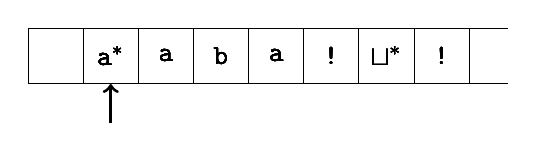
\begin{tikzpicture}

\draw (0.35, 0.35)
  node[draw, line width=0.01cm, , color=black,
       rounded corners=0cm, inner sep=0cm] {

\begin{minipage}[t][0.7cm]{0.7cm}
\mbox{}

\end{minipage}

};\draw (0.35, 0.35) node[color=black] {\texttt{\DOLLAR}};
\draw (1.0499999999999998, 0.35)
  node[draw, line width=0.01cm, , color=black,
       rounded corners=0cm, inner sep=0cm] {

\begin{minipage}[t][0.7cm]{0.7cm}
\mbox{}

\end{minipage}

};\draw (1.0499999999999998, 0.35) node[color=black] {\texttt{a$^*$}};
\draw (1.7499999999999998, 0.35)
  node[draw, line width=0.01cm, , color=black,
       rounded corners=0cm, inner sep=0cm] {

\begin{minipage}[t][0.7cm]{0.7cm}
\mbox{}

\end{minipage}

};\draw (1.7499999999999998, 0.35) node[color=black] {\texttt{a}};
\draw (2.4499999999999997, 0.35)
  node[draw, line width=0.01cm, , color=black,
       rounded corners=0cm, inner sep=0cm] {

\begin{minipage}[t][0.7cm]{0.7cm}
\mbox{}

\end{minipage}

};\draw (2.4499999999999997, 0.35) node[color=black] {\texttt{b}};
\draw (3.15, 0.35)
  node[draw, line width=0.01cm, , color=black,
       rounded corners=0cm, inner sep=0cm] {

\begin{minipage}[t][0.7cm]{0.7cm}
\mbox{}

\end{minipage}

};\draw (3.15, 0.35) node[color=black] {\texttt{a}};
\draw (3.85, 0.35)
  node[draw, line width=0.01cm, , color=black,
       rounded corners=0cm, inner sep=0cm] {

\begin{minipage}[t][0.7cm]{0.7cm}
\mbox{}

\end{minipage}

};\draw (3.85, 0.35) node[color=black] {\texttt{!}};
\draw (4.550000000000001, 0.35)
  node[draw, line width=0.01cm, , color=black,
       rounded corners=0cm, inner sep=0cm] {

\begin{minipage}[t][0.7cm]{0.7cm}
\mbox{}

\end{minipage}

};\draw (4.550000000000001, 0.35) node[color=black] {\texttt{$\sqcup^*$}};
\draw (5.25, 0.35)
  node[draw, line width=0.01cm, , color=black,
       rounded corners=0cm, inner sep=0cm] {

\begin{minipage}[t][0.7cm]{0.7cm}
\mbox{}

\end{minipage}

};\draw (5.25, 0.35) node[color=black] {\texttt{!}};
\draw (0.35, 0.35)
  node[draw, line width=0.01cm, , color=black,
       rounded corners=0cm, inner sep=0cm] {

\begin{minipage}[t][0.7cm]{0.7cm}
\mbox{}

\end{minipage}

};\draw (0.35, 0.35) node[color=black] {\texttt{\DOLLAR}};
\draw (1.0499999999999998, 0.35)
  node[draw, line width=0.01cm, , color=black,
       rounded corners=0cm, inner sep=0cm] {

\begin{minipage}[t][0.7cm]{0.7cm}
\mbox{}

\end{minipage}

};\draw (1.0499999999999998, 0.35) node[color=black] {\texttt{a$^*$}};
\draw (1.7499999999999998, 0.35)
  node[draw, line width=0.01cm, , color=black,
       rounded corners=0cm, inner sep=0cm] {

\begin{minipage}[t][0.7cm]{0.7cm}
\mbox{}

\end{minipage}

};\draw (1.7499999999999998, 0.35) node[color=black] {\texttt{a}};
\draw (2.4499999999999997, 0.35)
  node[draw, line width=0.01cm, , color=black,
       rounded corners=0cm, inner sep=0cm] {

\begin{minipage}[t][0.7cm]{0.7cm}
\mbox{}

\end{minipage}

};\draw (2.4499999999999997, 0.35) node[color=black] {\texttt{b}};
\draw (3.15, 0.35)
  node[draw, line width=0.01cm, , color=black,
       rounded corners=0cm, inner sep=0cm] {

\begin{minipage}[t][0.7cm]{0.7cm}
\mbox{}

\end{minipage}

};\draw (3.15, 0.35) node[color=black] {\texttt{a}};
\draw (3.85, 0.35)
  node[draw, line width=0.01cm, , color=black,
       rounded corners=0cm, inner sep=0cm] {

\begin{minipage}[t][0.7cm]{0.7cm}
\mbox{}

\end{minipage}

};\draw (3.85, 0.35) node[color=black] {\texttt{!}};
\draw (4.550000000000001, 0.35)
  node[draw, line width=0.01cm, , color=black,
       rounded corners=0cm, inner sep=0cm] {

\begin{minipage}[t][0.7cm]{0.7cm}
\mbox{}

\end{minipage}

};\draw (4.550000000000001, 0.35) node[color=black] {\texttt{$\sqcup^*$}};
\draw (5.25, 0.35)
  node[draw, line width=0.01cm, , color=black,
       rounded corners=0cm, inner sep=0cm] {

\begin{minipage}[t][0.7cm]{0.7cm}
\mbox{}

\end{minipage}

};\draw (5.25, 0.35) node[color=black] {\texttt{!}};
\draw (0.35, 0.35)
  node[draw, line width=0.01cm, , color=black,
       rounded corners=0cm, inner sep=0cm] {

\begin{minipage}[t][0.7cm]{0.7cm}
\mbox{}

\end{minipage}

};\draw (0.35, 0.35) node[color=black] {\texttt{\DOLLAR}};
\draw (1.0499999999999998, 0.35)
  node[draw, line width=0.01cm, , color=black,
       rounded corners=0cm, inner sep=0cm] {

\begin{minipage}[t][0.7cm]{0.7cm}
\mbox{}

\end{minipage}

};\draw (1.0499999999999998, 0.35) node[color=black] {\texttt{a$^*$}};
\draw (1.7499999999999998, 0.35)
  node[draw, line width=0.01cm, , color=black,
       rounded corners=0cm, inner sep=0cm] {

\begin{minipage}[t][0.7cm]{0.7cm}
\mbox{}

\end{minipage}

};\draw (1.7499999999999998, 0.35) node[color=black] {\texttt{a}};
\draw (2.4499999999999997, 0.35)
  node[draw, line width=0.01cm, , color=black,
       rounded corners=0cm, inner sep=0cm] {

\begin{minipage}[t][0.7cm]{0.7cm}
\mbox{}

\end{minipage}

};\draw (2.4499999999999997, 0.35) node[color=black] {\texttt{b}};
\draw (3.15, 0.35)
  node[draw, line width=0.01cm, , color=black,
       rounded corners=0cm, inner sep=0cm] {

\begin{minipage}[t][0.7cm]{0.7cm}
\mbox{}

\end{minipage}

};\draw (3.15, 0.35) node[color=black] {\texttt{a}};
\draw (3.85, 0.35)
  node[draw, line width=0.01cm, , color=black,
       rounded corners=0cm, inner sep=0cm] {

\begin{minipage}[t][0.7cm]{0.7cm}
\mbox{}

\end{minipage}

};\draw (3.85, 0.35) node[color=black] {\texttt{!}};
\draw (4.550000000000001, 0.35)
  node[draw, line width=0.01cm, , color=black,
       rounded corners=0cm, inner sep=0cm] {

\begin{minipage}[t][0.7cm]{0.7cm}
\mbox{}

\end{minipage}

};\draw (4.550000000000001, 0.35) node[color=black] {\texttt{$\sqcup^*$}};
\draw (5.25, 0.35)
  node[draw, line width=0.01cm, , color=black,
       rounded corners=0cm, inner sep=0cm] {

\begin{minipage}[t][0.7cm]{0.7cm}
\mbox{}

\end{minipage}

};\draw (5.25, 0.35) node[color=black] {\texttt{!}};
\draw (0.35, 0.35)
  node[draw, line width=0.01cm, , color=black,
       rounded corners=0cm, inner sep=0cm] {

\begin{minipage}[t][0.7cm]{0.7cm}
\mbox{}

\end{minipage}

};\draw (0.35, 0.35) node[color=black] {\texttt{\DOLLAR}};
\draw (1.0499999999999998, 0.35)
  node[draw, line width=0.01cm, , color=black,
       rounded corners=0cm, inner sep=0cm] {

\begin{minipage}[t][0.7cm]{0.7cm}
\mbox{}

\end{minipage}

};\draw (1.0499999999999998, 0.35) node[color=black] {\texttt{a$^*$}};
\draw (1.7499999999999998, 0.35)
  node[draw, line width=0.01cm, , color=black,
       rounded corners=0cm, inner sep=0cm] {

\begin{minipage}[t][0.7cm]{0.7cm}
\mbox{}

\end{minipage}

};\draw (1.7499999999999998, 0.35) node[color=black] {\texttt{a}};
\draw (2.4499999999999997, 0.35)
  node[draw, line width=0.01cm, , color=black,
       rounded corners=0cm, inner sep=0cm] {

\begin{minipage}[t][0.7cm]{0.7cm}
\mbox{}

\end{minipage}

};\draw (2.4499999999999997, 0.35) node[color=black] {\texttt{b}};
\draw (3.15, 0.35)
  node[draw, line width=0.01cm, , color=black,
       rounded corners=0cm, inner sep=0cm] {

\begin{minipage}[t][0.7cm]{0.7cm}
\mbox{}

\end{minipage}

};\draw (3.15, 0.35) node[color=black] {\texttt{a}};
\draw (3.85, 0.35)
  node[draw, line width=0.01cm, , color=black,
       rounded corners=0cm, inner sep=0cm] {

\begin{minipage}[t][0.7cm]{0.7cm}
\mbox{}

\end{minipage}

};\draw (3.85, 0.35) node[color=black] {\texttt{!}};
\draw (4.550000000000001, 0.35)
  node[draw, line width=0.01cm, , color=black,
       rounded corners=0cm, inner sep=0cm] {

\begin{minipage}[t][0.7cm]{0.7cm}
\mbox{}

\end{minipage}

};\draw (4.550000000000001, 0.35) node[color=black] {\texttt{$\sqcup^*$}};
\draw (5.25, 0.35)
  node[draw, line width=0.01cm, , color=black,
       rounded corners=0cm, inner sep=0cm] {

\begin{minipage}[t][0.7cm]{0.7cm}
\mbox{}

\end{minipage}

};\draw (5.25, 0.35) node[color=black] {\texttt{!}};
\draw (0.35, 0.35)
  node[draw, line width=0.01cm, , color=black,
       rounded corners=0cm, inner sep=0cm] {

\begin{minipage}[t][0.7cm]{0.7cm}
\mbox{}

\end{minipage}

};\draw (0.35, 0.35) node[color=black] {\texttt{\DOLLAR}};
\draw (1.0499999999999998, 0.35)
  node[draw, line width=0.01cm, , color=black,
       rounded corners=0cm, inner sep=0cm] {

\begin{minipage}[t][0.7cm]{0.7cm}
\mbox{}

\end{minipage}

};\draw (1.0499999999999998, 0.35) node[color=black] {\texttt{a$^*$}};
\draw (1.7499999999999998, 0.35)
  node[draw, line width=0.01cm, , color=black,
       rounded corners=0cm, inner sep=0cm] {

\begin{minipage}[t][0.7cm]{0.7cm}
\mbox{}

\end{minipage}

};\draw (1.7499999999999998, 0.35) node[color=black] {\texttt{a}};
\draw (2.4499999999999997, 0.35)
  node[draw, line width=0.01cm, , color=black,
       rounded corners=0cm, inner sep=0cm] {

\begin{minipage}[t][0.7cm]{0.7cm}
\mbox{}

\end{minipage}

};\draw (2.4499999999999997, 0.35) node[color=black] {\texttt{b}};
\draw (3.15, 0.35)
  node[draw, line width=0.01cm, , color=black,
       rounded corners=0cm, inner sep=0cm] {

\begin{minipage}[t][0.7cm]{0.7cm}
\mbox{}

\end{minipage}

};\draw (3.15, 0.35) node[color=black] {\texttt{a}};
\draw (3.85, 0.35)
  node[draw, line width=0.01cm, , color=black,
       rounded corners=0cm, inner sep=0cm] {

\begin{minipage}[t][0.7cm]{0.7cm}
\mbox{}

\end{minipage}

};\draw (3.85, 0.35) node[color=black] {\texttt{!}};
\draw (4.550000000000001, 0.35)
  node[draw, line width=0.01cm, , color=black,
       rounded corners=0cm, inner sep=0cm] {

\begin{minipage}[t][0.7cm]{0.7cm}
\mbox{}

\end{minipage}

};\draw (4.550000000000001, 0.35) node[color=black] {\texttt{$\sqcup^*$}};
\draw (5.25, 0.35)
  node[draw, line width=0.01cm, , color=black,
       rounded corners=0cm, inner sep=0cm] {

\begin{minipage}[t][0.7cm]{0.7cm}
\mbox{}

\end{minipage}

};\draw (5.25, 0.35) node[color=black] {\texttt{!}};
\draw (0.35, 0.35)
  node[draw, line width=0.01cm, , color=black,
       rounded corners=0cm, inner sep=0cm] {

\begin{minipage}[t][0.7cm]{0.7cm}
\mbox{}

\end{minipage}

};\draw (0.35, 0.35) node[color=black] {\texttt{\DOLLAR}};
\draw (1.0499999999999998, 0.35)
  node[draw, line width=0.01cm, , color=black,
       rounded corners=0cm, inner sep=0cm] {

\begin{minipage}[t][0.7cm]{0.7cm}
\mbox{}

\end{minipage}

};\draw (1.0499999999999998, 0.35) node[color=black] {\texttt{a$^*$}};
\draw (1.7499999999999998, 0.35)
  node[draw, line width=0.01cm, , color=black,
       rounded corners=0cm, inner sep=0cm] {

\begin{minipage}[t][0.7cm]{0.7cm}
\mbox{}

\end{minipage}

};\draw (1.7499999999999998, 0.35) node[color=black] {\texttt{a}};
\draw (2.4499999999999997, 0.35)
  node[draw, line width=0.01cm, , color=black,
       rounded corners=0cm, inner sep=0cm] {

\begin{minipage}[t][0.7cm]{0.7cm}
\mbox{}

\end{minipage}

};\draw (2.4499999999999997, 0.35) node[color=black] {\texttt{b}};
\draw (3.15, 0.35)
  node[draw, line width=0.01cm, , color=black,
       rounded corners=0cm, inner sep=0cm] {

\begin{minipage}[t][0.7cm]{0.7cm}
\mbox{}

\end{minipage}

};\draw (3.15, 0.35) node[color=black] {\texttt{a}};
\draw (3.85, 0.35)
  node[draw, line width=0.01cm, , color=black,
       rounded corners=0cm, inner sep=0cm] {

\begin{minipage}[t][0.7cm]{0.7cm}
\mbox{}

\end{minipage}

};\draw (3.85, 0.35) node[color=black] {\texttt{!}};
\draw (4.550000000000001, 0.35)
  node[draw, line width=0.01cm, , color=black,
       rounded corners=0cm, inner sep=0cm] {

\begin{minipage}[t][0.7cm]{0.7cm}
\mbox{}

\end{minipage}

};\draw (4.550000000000001, 0.35) node[color=black] {\texttt{$\sqcup^*$}};
\draw (5.25, 0.35)
  node[draw, line width=0.01cm, , color=black,
       rounded corners=0cm, inner sep=0cm] {

\begin{minipage}[t][0.7cm]{0.7cm}
\mbox{}

\end{minipage}

};\draw (5.25, 0.35) node[color=black] {\texttt{!}};
\draw (0.35, 0.35)
  node[draw, line width=0.01cm, , color=black,
       rounded corners=0cm, inner sep=0cm] {

\begin{minipage}[t][0.7cm]{0.7cm}
\mbox{}

\end{minipage}

};\draw (0.35, 0.35) node[color=black] {\texttt{\DOLLAR}};
\draw (1.0499999999999998, 0.35)
  node[draw, line width=0.01cm, , color=black,
       rounded corners=0cm, inner sep=0cm] {

\begin{minipage}[t][0.7cm]{0.7cm}
\mbox{}

\end{minipage}

};\draw (1.0499999999999998, 0.35) node[color=black] {\texttt{a$^*$}};
\draw (1.7499999999999998, 0.35)
  node[draw, line width=0.01cm, , color=black,
       rounded corners=0cm, inner sep=0cm] {

\begin{minipage}[t][0.7cm]{0.7cm}
\mbox{}

\end{minipage}

};\draw (1.7499999999999998, 0.35) node[color=black] {\texttt{a}};
\draw (2.4499999999999997, 0.35)
  node[draw, line width=0.01cm, , color=black,
       rounded corners=0cm, inner sep=0cm] {

\begin{minipage}[t][0.7cm]{0.7cm}
\mbox{}

\end{minipage}

};\draw (2.4499999999999997, 0.35) node[color=black] {\texttt{b}};
\draw (3.15, 0.35)
  node[draw, line width=0.01cm, , color=black,
       rounded corners=0cm, inner sep=0cm] {

\begin{minipage}[t][0.7cm]{0.7cm}
\mbox{}

\end{minipage}

};\draw (3.15, 0.35) node[color=black] {\texttt{a}};
\draw (3.85, 0.35)
  node[draw, line width=0.01cm, , color=black,
       rounded corners=0cm, inner sep=0cm] {

\begin{minipage}[t][0.7cm]{0.7cm}
\mbox{}

\end{minipage}

};\draw (3.85, 0.35) node[color=black] {\texttt{!}};
\draw (4.550000000000001, 0.35)
  node[draw, line width=0.01cm, , color=black,
       rounded corners=0cm, inner sep=0cm] {

\begin{minipage}[t][0.7cm]{0.7cm}
\mbox{}

\end{minipage}

};\draw (4.550000000000001, 0.35) node[color=black] {\texttt{$\sqcup^*$}};
\draw (5.25, 0.35)
  node[draw, line width=0.01cm, , color=black,
       rounded corners=0cm, inner sep=0cm] {

\begin{minipage}[t][0.7cm]{0.7cm}
\mbox{}

\end{minipage}

};\draw (5.25, 0.35) node[color=black] {\texttt{!}};
\draw (0.35, 0.35)
  node[draw, line width=0.01cm, , color=black,
       rounded corners=0cm, inner sep=0cm] {

\begin{minipage}[t][0.7cm]{0.7cm}
\mbox{}

\end{minipage}

};\draw (0.35, 0.35) node[color=black] {\texttt{\DOLLAR}};
\draw (1.0499999999999998, 0.35)
  node[draw, line width=0.01cm, , color=black,
       rounded corners=0cm, inner sep=0cm] {

\begin{minipage}[t][0.7cm]{0.7cm}
\mbox{}

\end{minipage}

};\draw (1.0499999999999998, 0.35) node[color=black] {\texttt{a$^*$}};
\draw (1.7499999999999998, 0.35)
  node[draw, line width=0.01cm, , color=black,
       rounded corners=0cm, inner sep=0cm] {

\begin{minipage}[t][0.7cm]{0.7cm}
\mbox{}

\end{minipage}

};\draw (1.7499999999999998, 0.35) node[color=black] {\texttt{a}};
\draw (2.4499999999999997, 0.35)
  node[draw, line width=0.01cm, , color=black,
       rounded corners=0cm, inner sep=0cm] {

\begin{minipage}[t][0.7cm]{0.7cm}
\mbox{}

\end{minipage}

};\draw (2.4499999999999997, 0.35) node[color=black] {\texttt{b}};
\draw (3.15, 0.35)
  node[draw, line width=0.01cm, , color=black,
       rounded corners=0cm, inner sep=0cm] {

\begin{minipage}[t][0.7cm]{0.7cm}
\mbox{}

\end{minipage}

};\draw (3.15, 0.35) node[color=black] {\texttt{a}};
\draw (3.85, 0.35)
  node[draw, line width=0.01cm, , color=black,
       rounded corners=0cm, inner sep=0cm] {

\begin{minipage}[t][0.7cm]{0.7cm}
\mbox{}

\end{minipage}

};\draw (3.85, 0.35) node[color=black] {\texttt{!}};
\draw (4.550000000000001, 0.35)
  node[draw, line width=0.01cm, , color=black,
       rounded corners=0cm, inner sep=0cm] {

\begin{minipage}[t][0.7cm]{0.7cm}
\mbox{}

\end{minipage}

};\draw (4.550000000000001, 0.35) node[color=black] {\texttt{$\sqcup^*$}};
\draw (5.25, 0.35)
  node[draw, line width=0.01cm, , color=black,
       rounded corners=0cm, inner sep=0cm] {

\begin{minipage}[t][0.7cm]{0.7cm}
\mbox{}

\end{minipage}

};\draw (5.25, 0.35) node[color=black] {\texttt{!}};\draw[line width=0.01cm,black] (5.6000000000000005,0.7) to  (6.1000000000000005,0.7);
\draw[line width=0.01cm,black] (5.6000000000000005,0.0) to  (6.1000000000000005,0.0);
\draw[line width=0.04cm,black,->] (1.05,-0.51) to  (1.05,-0.01);
\end{tikzpicture}

\end{center}



Note that the value at the top of the stack is the one removed.
Now if I remove a value again, the stack would look like this:

{\small \begin{console}[frame=single,fontsize=\small]
[student@localhost 350-hashtable] g++ main.cpp; ./a.out
hash of
42: 42
42: 42
-1: 18446744073709551615
3.14: 5464867211497793177
0.0: 6369015886390043782
'a': 97
true: 1
"hello world": 5577293430985752569
\end{console}
}


A stack is self-organizing in the sense that you can put values
into the stack, but you do not tell the stack \textit{where} to put the value.
The stack will decide where to put it.
Also, you can retrieve a value from the stack, but you don't say which value.
The ordering of the values is such that
the value taken out from the stack is the last value put into the stack.
This is just like a stack of plates:
the plate to take off the stack is the one on top and is
the last plate placed into the stack.

Putting a value into the stack is called \textbf{pushing} a value onto the stack.
The value that a user can see when he's looking at a stack is the
value on top of the stack.
This is a technical term: the value on top of the stack is called
the \defterm{top} of the stack.
Removing a value out of the stack is called \defterm{popping} the stack.
Frequently, the value popped off the stack is returned.

What else can you do with a stack?
\begin{tightlist}
  \li Asking for the size of the stack
  \li Asking if the stack is empty
  \li Clearing the stack
\end{tightlist}
Etc.
If you pop an empty stack, you should probably thrown an exception.


You can (and should) think of a stack as a memory device.
When you push something onto the stack,
you're saying to the stack \lq\lq Hang on to this please. I'll want it back later.''
When you take something out of a stack, you're basically
saying to the stack \lq\lq Give me the last thing I handed to you.''

Now for the implementation of stack ...

Note that the stack is very \lq\lq linear''. 
So it's not too surprising that you can implement it using arrays (dynamic or static)
and linked list.
Now note that the operation on a stack is at \lq\lq one end'' of the stack.

\begin{ex}
If you implement a stack using an array, which end of the array should be
used (the slot at index 0 of the opposite) for the top of the stack?
Why?
What is the runtime for push and pop?
(If the maximum size of the stack is small, then an array will do.)
\qed
\end{ex}

\begin{ex}
If the stack is huge, then a linked list can be used.
Should we use a singly or a doubly linked list?
Why?
What is the runtime for push and pop?
\qed
\end{ex}


\begin{ex}
Implement the stack (to contain integers) so that you can do this:
\begin{Verbatim}[frame=single,fontsize=\footnotesize]
Stack stack;
std::cout << stack.size() << '\n';     // prints 0
stack.push(3);                      
std::cout << stack << '\n';            // prints [3]
stack.push(6);
std::cout << stack << '\n';            // prints [6, 3] 
stack.push(1);
std::cout << stack << '\n';            // prints [1, 6, 3]
std::cout << stack.top() << '\n';      // prints [1, 6, 3]
std::cout << stack.is_empty() << '\n'; // prints 0 
int t = stack.pop();
std::cout << t << '\n';                // prints 1
std::cout << stack << '\n';            // prints [6, 3]
\end{Verbatim}
\end{ex}

\begin{ex}
Once you're done with the above, change it to a class template so that the above
code becomes:
\begin{Verbatim}[frame=single,fontsize=\footnotesize]
Stack< int > stack;
...
\end{Verbatim}
You can also have a stack of doubles:
\begin{Verbatim}[frame=single,fontsize=\footnotesize]
Stack< double > stack;
...
\end{Verbatim}
\end{ex}


\begin{ex}
Of course there are standard class operations you want:
\begin{Verbatim}[frame=single,fontsize=\footnotesize]
Stack< int > stack0;
Stack< int > stack1(stack0);
std::cout << (stack0 == stack1) << std::endl;
stack1 = stack0;
\end{Verbatim}
\end{ex}
